\noindent In den Kapiteln \ref{seven} und \ref{eight} werden zwei- und mehrdimensionale Datens\"{a}tze und Zufallsvariablen vorgestellt und beschrieben. Dabei wird die Kovarianz als Ma{\ss} f\"{u}r den Zusammenhang zweier Zufallsgr\"{o}{\ss}en diskutiert. Aufgrund einer fehlenden Normierung eignet sie sich jedoch nur bedingt zur Interpretation der Abh\"{a}ngigkeit. Eine geeignete Normierung liefert der Korrelationskoeffizient.\newline

\noindent Ist der Korrelationskoeffizient $\rho$ der Grundgesamtheit unbekannt, kann er auf Basis einer Stichprobe gesch\"{a}tzt werden. Die Bewertung dieser Sch\"{a}tzung erfolgt \"{u}ber einen Konfidenzbereich oder mithilfe eines Hypothesentests. Beide Verfahren werden in diesem Kapitel vorgestellt.

\subsection{Korrelationskoeffizient einer Stichprobe}

\noindent Der Korrelationskoeffizient r einer Stichprobe ist ein Ma{\ss} daf\"{u}r, wie \"{a}hnlich sich die zu untersuchenden Datens\"{a}tze oder Zufallsvariablen sind. Er beschreibt den Grad der linearen Abh\"{a}ngigkeit. Die Daten oder Zufallsvariablen k\"{o}nnen dabei kontinuierlich oder diskret sein.\newline

\noindent Zun\"{a}chst wird der Korrelationskoeffizient zweidimensionaler Stichproben definiert. Diese Definition wird anschlie{\ss}end auf M-dimensionale Zufallsvektoren erweitert.


\subsubsection{Korrelationskoeffizient r einer zweidimensionalen Stichprobe}

\noindent Um die Skalierungsabh\"{a}ngigkeit der Kovarianz zu eliminieren, kann sie normiert werden. Eine geeignete Normierung bildet der Korrelationskoeffizient r.

\begin{equation}\label{eq:tenone}
r=\dfrac{s_{xy}}{s_{x} \cdot s_{y}} =\dfrac{\dfrac{1}{N-1} \cdot \sum _{n=1}^{N}\left((x_{n} -\bar{x})\cdot (y_{n} -\bar{y})\right) }{\sqrt{\dfrac{1}{N-1} \cdot \sum _{n=1}^{N}(x_{n} -\bar{x})^{2}} \cdot \sqrt{\dfrac{1}{N-1} \cdot \sum _{n=1}^{N}(y_{n} -\bar{y})^{2}}}
\end{equation}

\noindent Durch die Normierung des Ausdrucks ist der Korrelationskoeffizient dimensionslos. Da die beiden Ausdr\"{u}cke f\"{u}r die Standardabweichungen $s_{x}$ und $s_{y}$ im Nenner immer positiv sind, ist das Vorzeichen des Korrelationskoeffizienten dasselbe wie das der Kovarianz. Da die Reihenfolge der Faktoren in Z\"{a}hler und Nenner beliebig ist, ist der Korrelationskoeffizient r unabh\"{a}ngig von der Reihenfolge der Stichprobengr\"{o}{\ss}en. 

\begin{equation}\label{eq:tentwo}
r=\dfrac{s_{xy}}{s_{x} \cdot s_{y}} =\dfrac{s_{yx}}{s_{y} \cdot s_{x}}
\end{equation}

\noindent Der Wert des Korrelationskoeffizienten r ist ein Ma{\ss} daf\"{u}r, wie stark die Zufallsvariablen linear voneinander abh\"{a}ngig sind. Bild \ref{fig:Korrelation1} stellt Stichproben mit unterschiedlichen Werten f\"{u}r den Korrelationskoeffizienten r dar.

\clearpage

\noindent 
\begin{figure}[H]
  \centerline{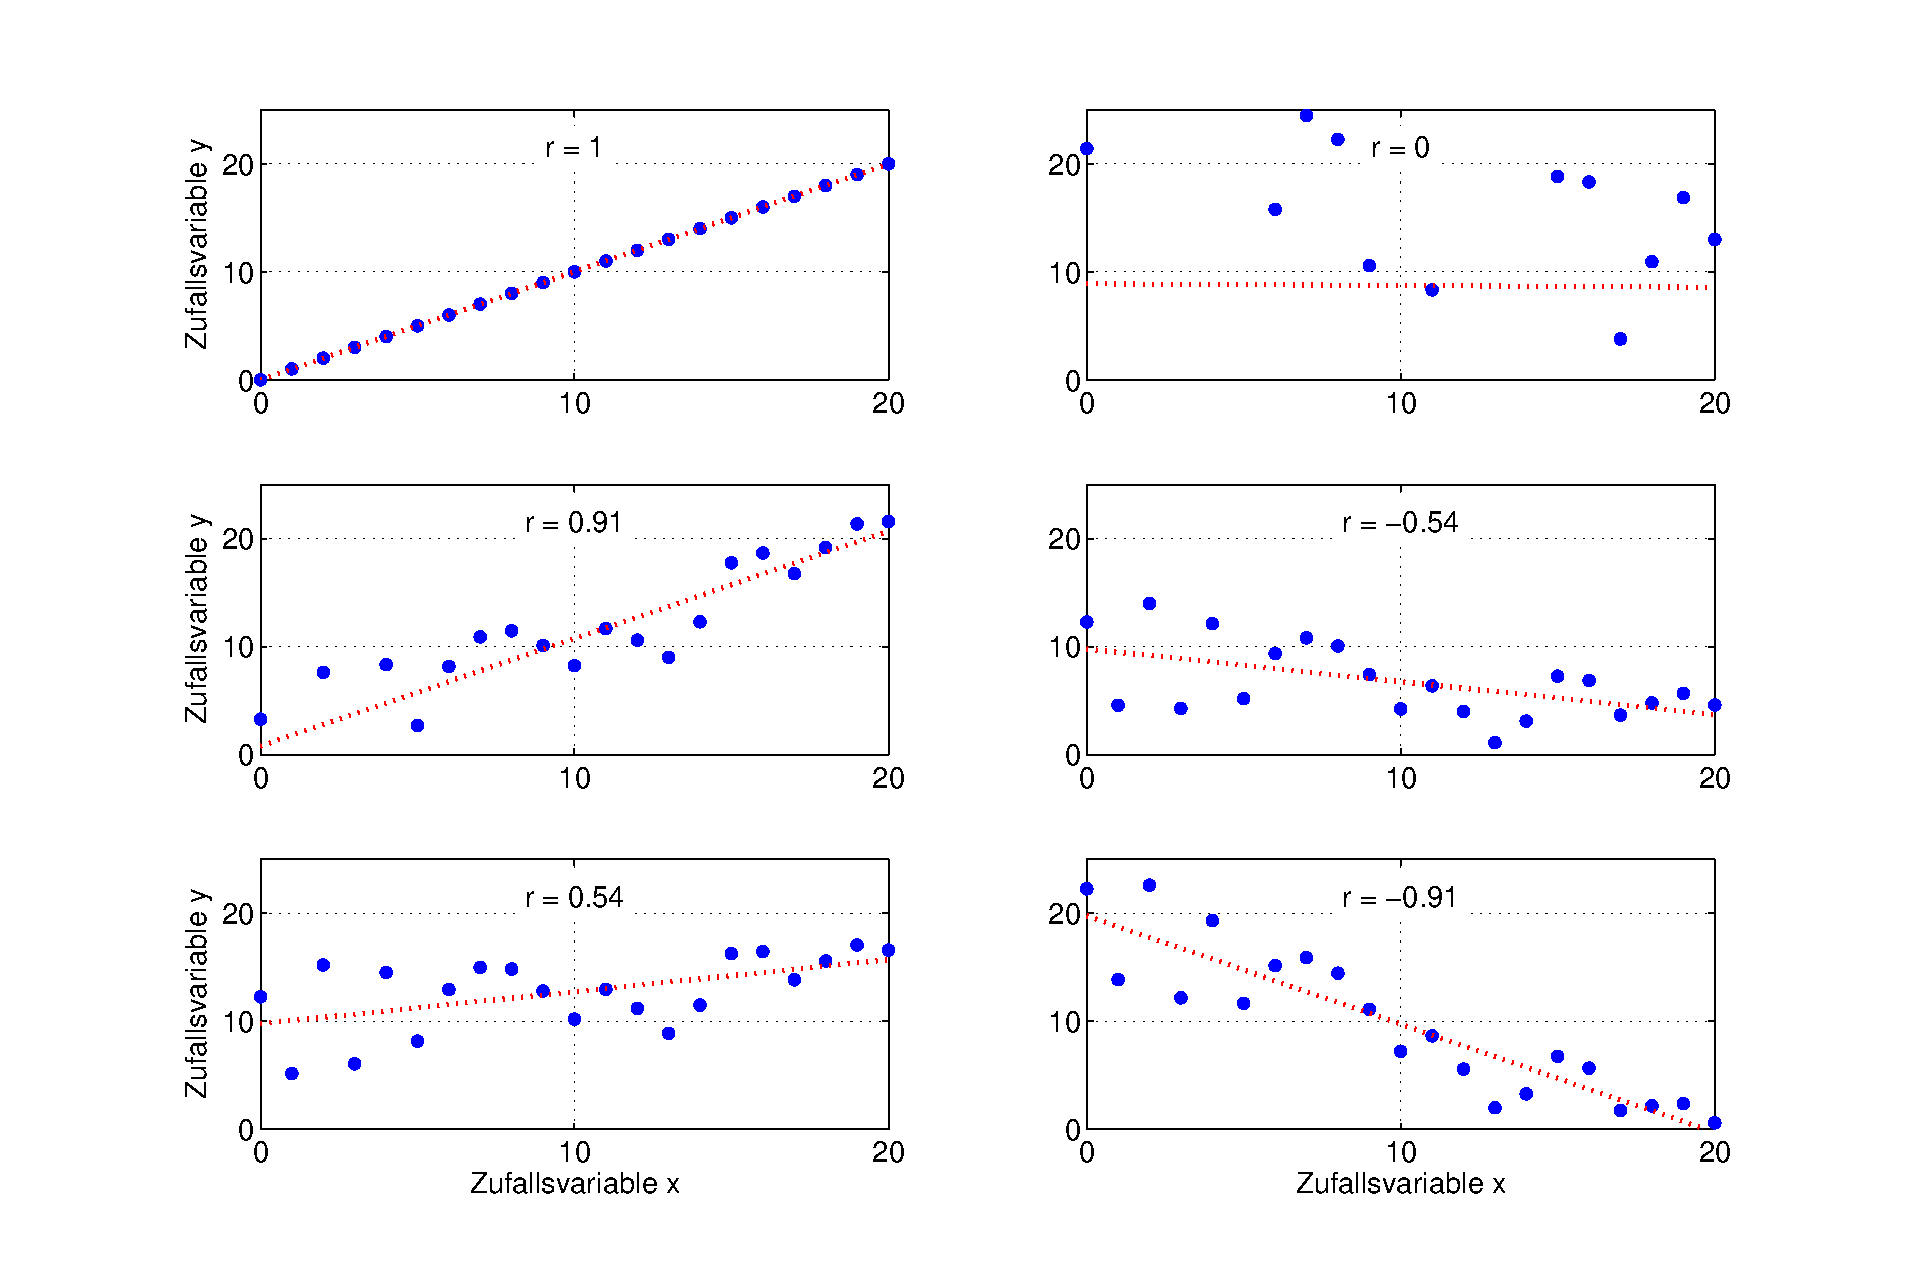
\includegraphics[width=1\textwidth]{Kapitel10/Bilder/image1}}
  \caption{Stichproben mit unterschiedlichen Werten f\"{u}r den Korrelationskoeffizienten r und der entsprechenden linearen Approximation}
  \label{fig:Korrelation1}
\end{figure}

\noindent In dem ersten Schaubild ist r = 1 und die Wertepaare liegen auf einer Geraden mit positiver Steigung. Im zweiten Diagramm ist der Korrelationskoeffizient r = 0, es existiert kein signifikanter Zusammenhang zwischen den Werten $x_{n}$ und $y_{n}$ der Stichprobe.\newline

\noindent Die \"{u}brigen Diagramme zeigen den Zusammenhang zwischen Streuungsdiagramm und Korrelationskoeffizient auf. Ein Betrag des Korrelationskoeffizienten r nahe 1 weist auf einen nahezu linearen Zusammenhang der beiden Gr\"{o}{\ss}en x und y hin. Je linearer der Zusammenhang ist, desto gr\"{o}{\ss}er ist der Betrag des Korrelationskoeffizienten r. Bei positivem Vorzeichen des Korrelationskoeffizienten steigen die Werte f\"{u}r y mit steigenden Werten f\"{u}r x an. Bei einem negativen Korrelationskoeffizienten fallen die Werte f\"{u}r y mit steigenden Werten f\"{u}r x. Tabelle \ref{tab:tenone} stellt die Eigenschaften des Korrelationskoeffizienten zusammen.

\begin{table}[H]
\setlength{\arrayrulewidth}{.1em}
\caption{Eigenschaften des Korrelationskoeffizienten}
\setlength{\fboxsep}{0pt}%
\colorbox{lightgray}{%
\arrayrulecolor{white}%
\begin{tabular}{ wc{8.3cm} | wc{8.3cm} }
\hline\xrowht{10pt}

\fontfamily{phv}\selectfont\textbf{Korrelationskoeffizient} &
\fontfamily{phv}\selectfont\textbf{Interpretation} \\ \hline \xrowht{10pt}

\fontfamily{phv}\selectfont{$r = 0$} & 
\fontfamily{phv}\selectfont{unkorrelierte Größen} \\ \hline\xrowht{10pt}

\multirow{2}{*}{\fontfamily{phv}\selectfont{$r > 0$}} & 
\fontfamily{phv}\selectfont{positive Korrelation} \\ \xrowht{10pt}

& 
\fontfamily{phv}\selectfont{gleichsinniger linearer Zusammenhang} \\ \hline\xrowht{10pt}

\multirow{2}{*}{\fontfamily{phv}\selectfont{$r < 0$}} & 
\fontfamily{phv}\selectfont{negative Korrelation} \\ \xrowht{10pt}

& 
\fontfamily{phv}\selectfont{gegensinniger linearer Zusammenhang} \\  \hline

\end{tabular}%
}
\label{tab:tenone}
\end{table}

\noindent Nimmt der Korrelationskoeffizient r den Wert 1 oder - 1 an, sind die Zufallsgr\"{o}{\ss}en linear voneinander abh\"{a}ngig und damit stark korreliert. F\"{u}r den Wert 0 des Korrelationskoeffizienten liegt keine lineare Abh\"{a}ngigkeit vor. Um die Korrelation auch zwischen diesen Eckpunkten einstufen zu k\"{o}nnen, wird die Korrelation je nach Betrag des Korrelationskoeffizienten r in eine schwache, mittlere oder starke Korrelation eingeteilt. Die einzelnen Intervalle sind in Tabelle \ref{tab:tentwo} aufgelistet.

\begin{table}[H]
\setlength{\arrayrulewidth}{.1em}
\caption{Einstufungen des Korrelationskoeffizienten}
\setlength{\fboxsep}{0pt}%
\colorbox{lightgray}{%
\arrayrulecolor{white}%
\begin{tabular}{ wc{8.3cm} | wc{8.3cm} }
\hline\xrowht{10pt}

\fontfamily{phv}\selectfont\textbf{Korrelationskoeffizient} &
\fontfamily{phv}\selectfont\textbf{Interpretation} \\ \hline \xrowht{10pt}

\fontfamily{phv}\selectfont{$\left | r \right | \leq 0.5$} & 
\fontfamily{phv}\selectfont{schwache Korrelation} \\ \hline\xrowht{10pt}

\fontfamily{phv}\selectfont{$\left | r \right | < 0.5 \leq 0.8$} & 
\fontfamily{phv}\selectfont{mittlere Korrelation} \\ \hline\xrowht{10pt}

\fontfamily{phv}\selectfont{$0.8 \leq \left | r \right |$} & 
\fontfamily{phv}\selectfont{starke Korrelation} \\  \hline

\end{tabular}%
}
\label{tab:tentwo}
\end{table}

\noindent Es sei noch einmal darauf hingewiesen, dass der Korrelationskoeffizient kein Ma{\ss} f\"{u}r die Abh\"{a}ngigkeit schlechthin ist, sondern ein Ma{\ss} f\"{u}r einen linearen Zusammenhang der beiden Zufallsvariablen. 

\noindent 
\begin{figure}[H]
  \centerline{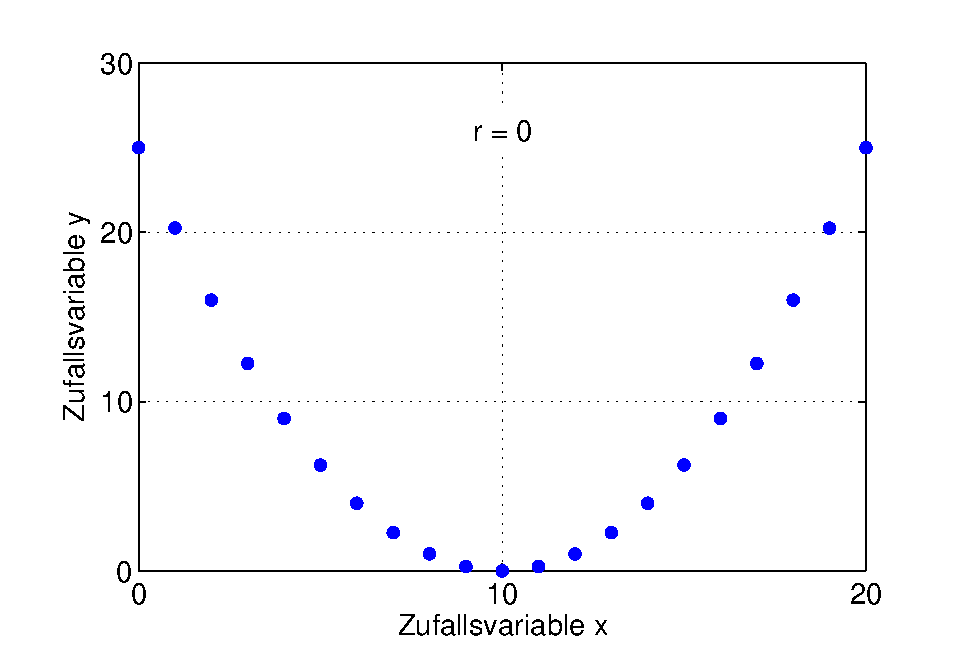
\includegraphics[width=0.5\textwidth]{Kapitel10/Bilder/image2}}
  \caption{Stichprobe unkorrelierter Werte mit einem Korrelationskoeffizienten r = 0}
  \label{fig:Korrelation2}
\end{figure}

\noindent Obwohl die beiden Zufallsvariablen einen quadratischen Zusammenhang aufweisen, ist ihre Korrelation r = 0. Es existiert kein linearer Zusammenhang zwischen den beiden Gr\"{o}{\ss}en.\bigskip

\noindent
\colorbox{lightgray}{%
\arrayrulecolor{white}%
\renewcommand\arraystretch{0.6}%
\begin{tabular}{ wl{16.5cm} }
{\fontfamily{phv}\selectfont
\noindent{Beispiel: Untersuchung einer synthetischen Faser}}
\end{tabular}%
}\medskip

\noindent Die gewonnenen Kenntnisse sollen an dem Beispiel einer zweidimensionalen Stichprobe verdeutlicht werden. Hierzu wird eine synthetische Faser mit einem festen Baumwollanteil untersucht. Es soll mittels Korrelation herausgefunden werden, ob zwischen der Zugfestigkeit dieser Faser und deren Trocknungszeit ein Zusammenhang besteht. Hierzu wurden 10 Faserproben analysiert, die in Tabelle \ref{tab:tenthree} aufgelistet sind.

\begin{table}[H]
\setlength{\arrayrulewidth}{.1em}
\caption{Daten zur Untersuchung einer synthetischen Faser}
\setlength{\fboxsep}{0pt}%
\colorbox{lightgray}{%
\arrayrulecolor{white}%
\begin{tabular}{ wc{1cm} | wc{3.1cm} | wc{3.1cm} | wc{1cm} | wc{3.3cm} | wc{3.3cm} }
\hline\xrowht{10pt}

\multirow{2}{*}{\fontfamily{phv}\selectfont\textbf{Nr.}} &
\fontfamily{phv}\selectfont\textbf{Trocknungszeit} &
\fontfamily{phv}\selectfont\textbf{Normierte} &
\multirow{2}{*}{\fontfamily{phv}\selectfont\textbf{Nr.}} &
\fontfamily{phv}\selectfont\textbf{Trocknungszeit} &
\fontfamily{phv}\selectfont\textbf{Normierte} \\

&
\fontfamily{phv}\selectfont\textbf{t / h} &
\fontfamily{phv}\selectfont\textbf{Zugfestigkeit R} &
&
\fontfamily{phv}\selectfont\textbf{t / h} &
\fontfamily{phv}\selectfont\textbf{Zugfestigkeit R} \\\hline \xrowht{10pt}

\fontfamily{phv}\selectfont{1} &
\fontfamily{phv}\selectfont{22.31} &
\fontfamily{phv}\selectfont{71.2467} &
\fontfamily{phv}\selectfont{6} &
\fontfamily{phv}\selectfont{25.48} &
\fontfamily{phv}\selectfont{72.9567} \\ \hline\xrowht{10pt}

\fontfamily{phv}\selectfont{2} &
\fontfamily{phv}\selectfont{4.48} &
\fontfamily{phv}\selectfont{73.7833} &
\fontfamily{phv}\selectfont{7} &
\fontfamily{phv}\selectfont{34.79} &
\fontfamily{phv}\selectfont{79.7900} \\ \hline\xrowht{10pt}

\fontfamily{phv}\selectfont{3} &
\fontfamily{phv}\selectfont{22.00} &
\fontfamily{phv}\selectfont{72.2867} &
\fontfamily{phv}\selectfont{8} &
\fontfamily{phv}\selectfont{41.71} &
\fontfamily{phv}\selectfont{81.3300} \\ \hline\xrowht{10pt}

\fontfamily{phv}\selectfont{4} &
\fontfamily{phv}\selectfont{26.29} &
\fontfamily{phv}\selectfont{75.4200} &
\fontfamily{phv}\selectfont{9} &
\fontfamily{phv}\selectfont{41.20} &
\fontfamily{phv}\selectfont{77.7067} \\ \hline\xrowht{10pt}

\fontfamily{phv}\selectfont{5} &
\fontfamily{phv}\selectfont{32.91} &
\fontfamily{phv}\selectfont{78.7000} &
\fontfamily{phv}\selectfont{10} &
\fontfamily{phv}\selectfont{43.34} &
\fontfamily{phv}\selectfont{80.3100} \\ \hline

\end{tabular}%
}
\label{tab:tenthree}
\end{table}

\noindent Um zun\"{a}chst einen \"{U}berblick \"{u}ber die Daten zu erhalten, werden die in Tabelle \ref{tab:tenthree} aufgelisteten Messwerte in einem Streudiagramm dargestellt.

\noindent 
\begin{figure}[H]
  \centerline{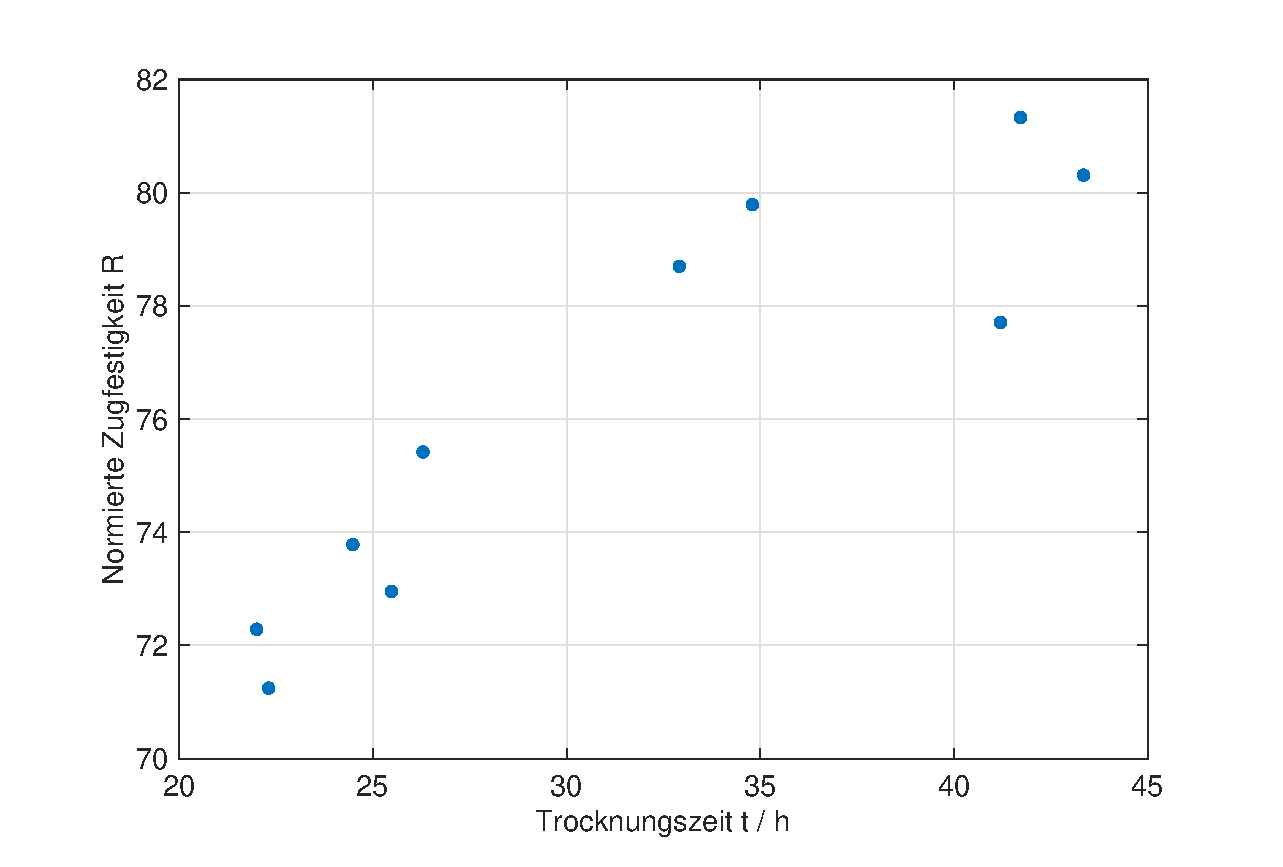
\includegraphics[width=0.5\textwidth]{Kapitel10/Bilder/image3}}
  \caption{Streudiagramm der Messwerte zur Untersuchung einer synthetischen Faser}
  \label{fig:ZugfestigkeitFasern}
\end{figure}

\noindent Die Kovarianz der Stichprobe berechnet sich zu

\begin{equation}\label{eq:tenthree}
s_{tR} =\dfrac{1}{N-1} \cdot \sum _{n=1}^{N}\left((t_{n} -\bar{t})\cdot (R_{n} -\bar{R})\right) = 28.2574
\end{equation}

\noindent Durch die Normierung mit

\begin{equation}\label{eq:tenfour}
s_{t}^{} =\sqrt{\dfrac{1}{N-1} \cdot \sum _{n=1}^{N}\left(t_{n} -\bar{t}\right)^{2}} =8.4240
\end{equation}

\noindent und

\begin{equation}\label{eq:tenfive}
s_{R} =\sqrt{\dfrac{1}{N-1} \cdot \sum _{n=1}^{N}(R_{n} -\bar{R})^{2}} =3.6697
\end{equation}

\noindent ergibt sich der Korrelationskoeffizient der Stichprobe zu

\begin{equation}\label{eq:tensix}
r=\dfrac{s_{tR}}{s_{t} \cdot s_{R}} =\dfrac{28.2574}{8.4240\cdot 3.6697} =0.9141
\end{equation}

\noindent Mit MATLAB errechnet sich dieser Wert durch

\lstinputlisting[caption = {}]{Kapitel10/mat1.m}

\noindent Entsprechend der Einstufung nach Tabelle 10.2 sind die Zugfestigkeit und die Trocknungszeit stark korreliert. Dieses Ergebnis entspricht der grafischen Bewertung von Bild 10.3, in dem zu erkennen ist, dass die Zugfestigkeit mit steigenden die Trocknungszeit zunimmt.\newline

\noindent In Python wird f\"{u}r multivariate Aufgaben typischerweise die Pandas-Datenstruktur Dataframe verwendet. F\"{u}r diesen Datentyp existiert die Methode corr, die die Korrelation zwischen Datenvektoren des Dataframes berechnet. Es entsteht eine Korrelationsmatrix, aus der das entsprechende Element ausgew\"{a}hlt wird.

\clearpage

\lstinputlisting[caption = {}]{Kapitel10/mat2.m}

\subsubsection{Korrelationsmatrix R einer multivariaten Stichprobe}

\noindent Die Darstellung multivariater Stichproben erfolgt mithilfe von Matrizen. Durch die Matrizen-Schreibweise ist es m\"{o}glich, die multivariate Bewertung auf die Bewertung von jeweils zwei Zufallsvariablen zur\"{u}ckzuf\"{u}hren. Diese Vorgehensweise wird bei der Einf\"{u}hrung der Kovarianzmatrix \textbf{S} in Abschnitt 8.2.2 beschrieben. Ein vergleichbares Vorgehen f\"{u}hrt zu einer Korrelationsmatrix \textbf{R}, die im Folgenden diskutiert wird. F\"{u}r jedes Paar $x_{j}$ und $x_{k}$ von Zufallsvariablen kann nach Gleichung \eqref{eq:tentwo} der zugeh\"{o}rige Korrelationskoeffizient $r_{jk}$ angegeben werden zu

\begin{equation}\label{eq:tenseven}
r_{jk} =\dfrac{s_{x_{j} x_{k}}}{s_{x_{j}} \cdot s_{x_{k}}} 
\end{equation}

\noindent Um die Wechselwirkung der Gr\"{o}{\ss}en miteinander paarweise zu beschreiben, wird eine Matrix von Korrelationskoeffizienten aufgestellt. Bei einer Anzahl von M Zufallsgr\"{o}{\ss}en ergibt sich eine Korrelationsmatrix \textbf{R} der Dimension M x M.

\begin{equation}\label{eq:teneight}
R=
\begin{pmatrix}
r_{11} & r_{12} & \dots & r_{1M}\\
r_{21} & r_{22} & \dots & r_{2M}\\
\dots & \dots & \dots & \dots \\
r_{M1} & r_{M2} & \dots & r_{MM}\\
\end{pmatrix} = 
\begin{pmatrix}
1 & r_{12} & \dots & r_{1M}\\
r_{2,1} & 1 & \dots & r_{2M}\\
\dots & \dots & \dots & \dots \\
r_{M1} & r_{M2} & \dots & 1\\
\end{pmatrix}
\end{equation}

\noindent Auf der Hauptdiagonale wird die Korrelation der Gr\"{o}{\ss}en mit sich selbst berechnet. Da der Zusammenhang zwischen jeder Gr\"{o}{\ss}e mit sich selbst streng linear ist, ist die Korrelation hier immer 1. Wegen der Symmetrie der Korrelation in Gleichung \eqref{eq:tentwo} ist die Korrelationsmatrix symmetrisch zur Hauptdiagonalen.

\clearpage

\subsection{Definition des Korrelationskoeffizienten \texorpdfstring{$\rho$}{Lg} der Grundgesamtheit}

\noindent In Kapitel \ref{five} und \ref{six} werden Verfahren vorgestellt, mit denen Vertrauensbereiche und Hypothesentests aufgebaut werden. Grundlage f\"{u}r diese Tests ist die Analyse einer Zufallsvariable, die den Zusammenhang zwischen der Stichprobe und der Grundgesamtheit herstellt. Um f\"{u}r den Korrelationskoeffizienten $\rho$ der Grundgesamtheit einen Konfidenzbereich angeben und einen Hypothesentest zur Signifikanzpr\"{u}fung durchf\"{u}hren zu k\"{o}nnen, wird in diesem Abschnitt der Korrelationskoeffizient der Grundgesamtheit eingef\"{u}hrt, und es werden die grundlegenden Eigenschaften des Korrelationskoeffizienten erl\"{a}utert.


\subsubsection{Korrelationskoeffizient \texorpdfstring{$\rho$}{Lg} der Grundgesamtheit von Wertepaaren}

\noindent Die in der zweidimensionalen Grundgesamtheit vorkommenden Mittelwerte $\mu_{x}$ und $\mu_{y}$ der beiden Zufallsvariablen x und y sind durch den Erwartungswert-Operator definiert zu

\begin{equation}\label{eq:tennine}
\mu _{x} =E(x)
\end{equation}

\noindent und

\begin{equation}\label{eq:tenten}
\mu _{y} =E(y)
\end{equation}

\noindent Die zugeh\"{o}rigen Varianzen der Grundgesamtheit errechnen sich aus

\begin{equation}\label{eq:teneleven}
\sigma _{x}^{2} =E\left((x-\mu _{x})^{2} \right)
\end{equation}

\noindent und

\begin{equation}\label{eq:tentwelve}
\sigma _{y}^{2} =E\left((y-\mu _{y})^{2} \right)
\end{equation}

\noindent Mit der Kovarianz $\sigma_{xy}$ der Zufallsgr\"{o}{\ss}en x und y

\begin{equation}\label{eq:tenthirteen}
\sigma _{xy} =E\left((x-\mu _{x})\cdot (y-\mu _{y})\right)=E(x\cdot y)-E(x)\cdot E(y)
\end{equation}

\noindent berechnet sich der Korrelationskoeffizient der Grundgesamtheit $\rho$ in Anlehnung an Gleichung \eqref{eq:tentwo} zu 

\begin{equation}\label{eq:tenfourteen}
\rho =\dfrac{\sigma _{xy}}{\sigma _{x} \cdot \sigma _{y}}
\end{equation}

\clearpage

\subsubsection{Korrelation der Grundgesamtheit einer multivariaten Stichprobe}

\noindent Analog zu der Korrelationsmatrix \textbf{R} aus Abschnitt 10.1 kann f\"{u}r jedes Paar $x_{j}$ und $x_{k}$ von Zufallsvariablen nach Gleichung \eqref{eq:tenseven} die Korrelation der Grundgesamtheit angegeben werden zu

\begin{equation}\label{eq:tenfifteen}
\rho _{jk} =\dfrac{\sigma _{x_{j} x_{k}}}{\sigma _{x_{j}} \cdot \sigma _{x_{k}}}
\end{equation}

\noindent Um die Wechselwirkung der Gr\"{o}{\ss}en miteinander paarweise zu beschreiben, wird eine Matrix von Korrelationskoeffizienten aufgestellt. Bei einer Anzahl von M Zufallsgr\"{o}{\ss}en ergibt sich eine Korrelationsmatrix der Dimension M x M.

\begin{equation}\label{eq:tensixteen}
P = 
\begin{pmatrix}
\rho _{11} & \rho _{12} & \dots & \rho _{1M}\\
\rho _{21} & \rho _{22} & \dots & \rho _{2M}\\
\dots & \dots & \dots & \dots\\
\rho _{M1} & \rho _{M2} & \dots & \rho _{MM}\\
\end{pmatrix}
\end{equation}

\noindent  Auf der Hauptdiagonale wird die Korrelation der Gr\"{o}{\ss}en mit sich selbst berechnet. Da der Zusammenhang zwischen jeder Gr\"{o}{\ss}en mit sich selbst streng linear ist, ist die Korrelation hier immer 1. Wegen der Symmetrie der Korrelation in Gleichung \eqref{eq:tenfifteen} ist die Korrelationsmatrix symmetrisch zur Hauptdiagonalen.

\subsubsection{Wertebereich des Korrelationskoeffizienten}

\noindent Der Korrelationskoeffizient $\rho$ liegt zwischen - 1 und 1.

\begin{equation}\label{eq:tenseventeen}
-1\le \rho \le 1
\end{equation}

\noindent F\"{u}r einen Beweis dieser Ungleichung werden die beiden standardnormalverteilten Zufallsgr\"{o}{\ss}en

\begin{equation}\label{eq:teneighteen}
z_{x} =\dfrac{x-\mu _{x}}{\sigma _{x}}
\end{equation}

\noindent und

\begin{equation}\label{eq:tennineteen}
z_{y} =\dfrac{y-\mu _{y}}{\sigma _{y}}
\end{equation}

\noindent zu der Zufallsgr\"{o}{\ss}e z

\begin{equation}\label{eq:tentwenty}
z=t\cdot z_{x} +z_{y}
\end{equation}

verrechnet. Der Erwartungswert der Zufallsvariablen z ergibt sich wegen der Standardnormalverteilung der Zufallsvariablen $z_{x}$ und $z_{y}$ zu

\begin{equation}\label{eq:tentwentyone}
E(z)=E(t\cdot z_{x} +z_{y})=t\cdot E(z_{x})+E(z_{y})=0
\end{equation}

\noindent F\"{u}r die Varianz der Zufallsvariablen folgt

\begin{equation}\label{eq:tentwentytwo}
E(z^{2})=E\left((t\cdot z_{x} +z_{y})^{2} \right)=t^{2} \cdot E(z_{x}^{2})+2\cdot t\cdot E(z_{x} \cdot z_{y})+E(z_{y}^{2})=t^{2} +2\cdot t\cdot E(z_{x} \cdot z_{y})+1
\end{equation}

\noindent Die Kovarianz der Zufallsgr\"{o}{\ss}en $z_{x}$ und $z_{y}$ l\"{a}sst sich umformen zu

\begin{equation}\label{eq:tentwentythree}
E(z_{x} \cdot z_{y})=E\left(\dfrac{x-\mu _{x}}{\sigma _{x}} \cdot \dfrac{y-\mu _{y}}{\sigma _{y}} \right)=\dfrac{1}{\sigma _{x} \cdot \sigma _{y}} \cdot E\left((x-\mu _{x})\cdot (y-\mu _{y})\right)=\dfrac{\sigma _{xy}}{\sigma _{x} \cdot \sigma _{y}} =\rho
\end{equation}

\noindent Damit folgt Gleichung \eqref{eq:tentwentytwo} zu

\begin{equation}\label{eq:tentwentyfour}
E(z^{2})=t^{2} +2\cdot t\cdot \rho +1
\end{equation}

\noindent Um zu zeigen, dass der Korrelationskoeffizient $\rho$ nie gr\"{o}{\ss}er als $\pm$ 1 wird, muss Gleichung \eqref{eq:tentwentyfour} umgeformt werden zu

\begin{equation}\label{eq:tentwentyfive}
E(z^{2})=(t+\rho)^{2} +1-\rho ^{2}
\end{equation}

\noindent Die Varianz einer Zufallsvariable ist als die Quadratsumme der Abst\"{a}nde der Einzelwerte zum Mittelwert definiert und damit immer gr\"{o}{\ss}er oder gleich null. Gleichung \eqref{eq:tentwentyfive} gen\"{u}gt somit der Ungleichung

\begin{equation}\label{eq:tentwentysix}
E(z^{2})=(t+\rho)^{2} +1-\rho ^{2} \ge 0
\end{equation}

\noindent Da der Teilausdruck $(t + \rho)^{2}$ stets gr\"{o}{\ss}er oder gleich 0 ist, muss dies auch f\"{u}r den Teilausdruck $1 - \rho^{2}$ gelten, um die Ungleichung \eqref{eq:tentwentysix} nicht zu verletzen. Daraus ergibt sich, dass

\begin{equation}\label{eq:tentwentyseven}
\rho ^{2} \le 1
\end{equation}

\noindent und damit

\begin{equation}\label{eq:tentwentyeight}
\rho \le \left|1\right|
\end{equation}

\noindent gilt.\newline

\noindent Damit ist bewiesen, dass der Korrelationskoeffizient $\rho$ zwischen - 1 und 1 liegt. 

\begin{equation}\label{eq:tentwentynine}
-1\le \rho \le 1
\end{equation}

\noindent Da der Korrelationskoeffizient der Stichprobe ein Sch\"{a}tzwert f\"{u}r den Korrelationskoeffizienten der Grundgesamtheit ist, gilt diese Ungleichung auch f\"{u}r den Korrelationskoeffizienten der Stichprobe.

\begin{equation}\label{eq:tenthirty}
-1\le r\le 1
\end{equation}

\clearpage

\subsubsection{Korrelation bei unabh\"{a}ngigen Zufallsvariablen}

\noindent Handelt es sich bei den Zufallsvariablen x und y um unabh\"{a}ngige Zufallsvariablen, gilt f\"{u}r deren Kovarianz $\sigma_{xy}$

\begin{equation}\label{eq:tenthirtyone}
\sigma _{xy} =E\left((x-\mu _{x})\cdot (y-\mu _{y})\right)=0
\end{equation}

\noindent Dieser Zusammenhang wird in Kapitel \ref{eight} bewiesen. Aus der Definition des Korrelationskoeffizienten

\begin{equation}\label{eq:tenthirtytwo}
\rho =\dfrac{\sigma _{xy}}{\sigma _{x} \cdot \sigma _{y}}
\end{equation}

\noindent folgt, dass dieser im Falle unabh\"{a}ngiger Zufallsvariablen ebenfalls zu null wird.

\begin{equation}\label{eq:tenthirtythree}
\rho =\dfrac{\sigma _{xy}}{\sigma _{x} \cdot \sigma _{y}} =\dfrac{0}{\sigma _{x} \cdot \sigma _{y}} =0
\end{equation}

\noindent Bei einer zweidimensionalen Normalverteilung gilt auch die Umkehrung dieses Satzes. Im Allgemeinen kann aber nicht davon ausgegangen werden, dass bei verschwindendem Korrelationskoeffizienten die Variablen unabh\"{a}ngig sind. Der Korrelationskoeffizient ist kein allgemeines Ma{\ss} f\"{u}r die Abh\"{a}ngigkeit, sondern ein Ma{\ss} f\"{u}r die lineare Abh\"{a}ngigkeit der beiden Gr\"{o}{\ss}en x und y. 

\subsubsection{Korrelation bei linearer Abh\"{a}ngigkeit der Zufallsvariablen}

\noindent Im Folgenden wird gezeigt, welchen Wert der Korrelationskoeffizient annimmt, wenn die Zufallsvariablen linear voneinander abh\"{a}ngig sind. In diesem Fall gilt die Beziehung

\begin{equation}\label{eq:tenthirtyfour}
y=b\cdot x+k
\end{equation}

\noindent Der Korrelationskoeffizient der beiden Zufallsvariablen x und y kann durch die Gleichung

\begin{equation}\label{eq:tenthirtyfive}
\rho =\dfrac{\sigma _{xy}}{\sigma _{x} \cdot \sigma _{y}}
\end{equation}

\noindent berechnet werden. Die Kovarianz $\sigma_{xy}$ wird durch den Erwartungswertoperator definiert 

\begin{equation}\label{eq:tenthirtysix}
\sigma _{xy} =E\left((x-\mu _{x})(y-\mu _{y})\right)
\end{equation}

\noindent Durch Einsetzen der Zufallsvariablen y aus Gleichung \eqref{eq:tenthirtyfour} in die Definitionsgleichung der Kovarianz folgt

\begin{equation}\label{eq:tenthirtyseven}
\begin{split}
E\left((x-\mu _{x})(y-\mu _{y})\right)& =E\left((x-E(x))\left(b\cdot x+k-E(b\cdot x+k)\right)\right)\\ 
& = E\left((x-E(x))\left(b\cdot (x-E(x))\right)\right)=b\cdot E\left((x-E(x))^{2} \right)
\end{split}
\end{equation}

\noindent Die Standardabweichung $\sigma_{x}$ und die Standardabweichung $\sigma_{y}$ lassen sich ebenfalls mithilfe des Erwartungswert-Operators ausdr\"{u}cken zu

\begin{equation}\label{eq:tenthirtyeight}
\sigma _{x} =\sqrt{E\left((x-\mu _{x})^{2} \right)} =\sqrt{E\left((x-E(x))^{2} \right)}
\end{equation}

\noindent und

\begin{equation}\label{eq:tenthirtynine}
\begin{split}
\sigma _{y} & =\sqrt{E\left((y-\mu _{y})^{2} \right)} =\sqrt{E\left(\left(b\cdot x+k-E(b\cdot x+k)\right)^{2} \right)} =\sqrt{E\left(\left(b\cdot (x-E(x))\right)^{2} \right)} \\
& = \left | b \right|\cdot\sqrt{E\left((x-E(x))^{2} \right)}
\end{split}
\end{equation}

\noindent Mit Gleichung \eqref{eq:tenthirtyseven}, Gleichung \eqref{eq:tenthirtyeight} und Gleichung \eqref{eq:tenthirtynine} folgt aus der Definitionsgleichung des Korrelationskoeffizienten $\rhoup$ 

\begin{equation}\label{eq:tenfourty}
\rho =\dfrac{\sigma _{xy}}{\sigma _{x} \cdot \sigma _{y}} =\dfrac{b\cdot E\left((x-E(x))^{2} \right)}{\sqrt{E\left((x-E(x))^{2} \right)} \cdot \left|b\right|\cdot \sqrt{E\left((x-E(x))^{2} \right)}} =\dfrac{b}{\left|b\right|}
\end{equation}

\noindent Der Korrelationskoeffizient $\rhoup$ weist damit f\"{u}r positive Werte b einen Wert von $\rho = 1$ auf, f\"{u}r einen negativen Koeffizienten b ergibt sich ein Wert von $\rho = - 1$. Der Korrelationskoeffizient $\rho$ nimmt damit bei exakt linearer Abh\"{a}ngigkeit den Betrag 1 an. F\"{u}r Abh\"{a}ngigkeiten, die sich approximativ als Gerade beschreiben lassen, ergibt sich ein Wert in den Grenzen von -1 und 1. Bei unabh\"{a}ngigen Zufallsvariablen besteht kein linearer Zusammenhang und der Korrelationskoeffizient nimmt den Wert 0 an, was in Abschnitt 10.2.3 gezeigt wird. Zus\"{a}tzlich kann \"{u}ber das Vorzeichen des Korrelationskoeffizienten eine Aussage dar\"{u}ber getroffen werden, ob mit steigenden Werten f\"{u}r die Zufallsvariable x die Werte der Zufallsvariablen ab- oder zunehmen.

\clearpage

\subsection{Bewertung des Korrelationskoeffizienten}

\noindent Die Verallgemeinerung der Korrelation einer Stichprobe auf die Grundgesamtheit erfordert die Bestimmung des Konfidenzbereiches und einen Hypothesentest f\"{u}r die Pr\"{u}fung der Korrelation auf Signifikanz.

\subsubsection{Bewertung des Korrelationskoeffizienten}

\noindent Aus der Literatur sind zwei unterschiedliche Zufallsvariablen zur Bewertung der Korrelationskoeffizienten bekannt [Fahr96]. \bigskip

{\fontfamily{phv}\selectfont
\noindent\textbf{Zufallsvariable f\"{u}r Korrelationskoeffizienten $\rho = 0$}}\smallskip

\noindent Liegt f\"{u}r eine Stichprobe mit dem Stichprobenumfang N die Korrelation r nahe dem Wert $\rho = 0$, sind die Zufallsvariablen x und y voraussichtlich statistisch unabh\"{a}ngig. F\"{u}r einen Test auf Unabh\"{a}ngigkeit wird die Hypothese $\rho = 0$ gepr\"{u}ft. F\"{u}r diesen Test wird die Zufallsvariable 

\begin{equation}\label{eq:tenfourtyone}
t=r\cdot \sqrt{\dfrac{N-2}{1-r^{2}}}  
\end{equation}

\noindent eingesetzt. Sie weist f\"{u}r $\rho = 0$ eine t-Verteilung mit N - 2 Freiheitsgraden auf.  \bigskip

{\fontfamily{phv}\selectfont
\noindent\textbf{Zufallsvariable f\"{u}r Korrelationskoeffizienten $\rho = \rho_{0}$}}\smallskip

\noindent Die Zufallsgr\"{o}{\ss}e t aus Gleichung \eqref{eq:tenfourtyone} geht von einer Unabh\"{a}ngigkeit der Zufallsgr\"{o}{\ss}en x und y aus. Soll die Korrelation $\rho$ auf einen Wert $\rho_{0} \neq 0$ gep\"{u}ft oder der Konfidenzbereich des Korrelationskoeffizienten angegeben werden, ist diese Voraussetzung nicht erf\"{u}llt. Aus diesem Grund wird in diesem Fall die Zufallsvariable 

\begin{equation}\label{eq:tenfourtytwo}
z=\dfrac{1}{2} \cdot \left(\ln \left(\dfrac{1+r}{1-r} \right)-\ln \left(\dfrac{1+\rho}{1-\rho} \right)\right)\cdot \sqrt{N-3} =\left(\tanh ^{-1} (r)-\tanh ^{-1} (\rho)\right)\cdot \sqrt{N-3} 
\end{equation}

\noindent f\"{u}r eine Bewertung des Korrelationskoeffizienten eingef\"{u}hrt. Sie ist f\"{u}r einen Stichprobenumfang $N > 25$ asymptotisch standardnormalverteilt.\newline

\noindent Auf Basis dieser Zufallsvariablen und ihren Verteilungen kann der Konfidenzbereich des Korrelationskoeffizienten $\rho$ bestimmt und mit einem Hypothesentest die Hypothese gepr\"{u}ft werden.


\subsubsection{Konfidenzbereich des Korrelationskoeffizienten}

\noindent Der Konfidenzbereich des Korrelationskoeffizienten wird \"{u}ber die standardnormalverteilte Zufallsvariable 

\begin{equation}\label{eq:tenfourtythree}
z=\dfrac{1}{2} \cdot \left(\ln \left(\dfrac{1+r}{1-r} \right)-\ln \left(\dfrac{1+\rho}{1-\rho} \right)\right)\cdot \sqrt{N-3} =\left(\tanh ^{-1} (r)-\tanh ^{-1} (\rho)\right)\cdot \sqrt{N-3}
\end{equation}

\noindent ausgewertet. Die Wahrscheinlichkeit $\gamma$, mit der die Variable z in dem Intervall $c_{1}$ ... $c_{2}$ liegt, ist definiert als

\begin{equation}\label{eq:tenfourtyfour}
P(c_{1} <z\le c_{2})=F(c_{2})-F(c_{1})=\gamma
\end{equation}

\noindent Bei Annahme eines symmetrischen Konfidenzbereiches ergeben sich die Konstanten $c_{1}$ und $c_{2}$ aus der inversen Standardnormalverteilung zu 

\begin{equation}\label{eq:tenfourtyfive}
c_{1} =F^{-1} \left(\dfrac{1-\gamma }{2} \right)
\end{equation}

\noindent und

\begin{equation}\label{eq:tenfourtysix}
c_{2} =F^{-1} \left(\dfrac{1+\gamma }{2} \right)
\end{equation}

\noindent Durch Umformungen ergibt sich ein Ausdruck f\"{u}r den Konfidenzbereich des Korrelationskoeffizienten $\rho$ der Grundgesamtheit.

\begin{equation}\label{eq:tenfourtyseven}
\begin{split}
\gamma  & = P\left(c_{1} <\left(\tanh ^{-1} (r)-\tanh ^{-1} (\rho)\right)\cdot \sqrt{N-3} \le c_{2} \right) \\ 
& = P\left(\dfrac{c_{1} }{\sqrt{N-3} } <\tanh ^{-1} (r)-\tanh ^{-1} (\rho )\le \dfrac{c_{2}}{\sqrt{N-3}} \right) \\ 
& = P\left(\dfrac{c_{1} }{\sqrt{N-3} } -\tanh ^{-1} (r)<-\tanh ^{-1} (\rho)\le \dfrac{c_{2}}{\sqrt{N-3}} -\tanh ^{-1} (r)\right)\\ 
& =P\left(\tanh ^{-1} (r)-\dfrac{c_{2} }{\sqrt{N-3}} <\tanh ^{-1} (\rho)\le \tanh ^{-1} (r)-\dfrac{c_{1}}{\sqrt{N-3}} \right)\\ 
& = P\left(\tanh \left(\tanh ^{-1} (r)-\dfrac{c_{2} }{\sqrt{N-3}} \right)<\rho \le \tanh \left(\tanh ^{-1} (r)-\dfrac{c_{1}}{\sqrt{N-3}} \right)\right)
\end{split}
\end{equation}

\noindent Mit der gew\"{a}hlten Wahrscheinlichkeit $\gamma$ liegt der Korrelationskoeffizienten $\rho$ der Grundgesamtheit in dem angegebenen Konfidenzintervall. Das Vorgehen zur Bestimmung des Konfidenzintervalls f\"{u}r den Korrelationskoeffizienten $\rho$ wird in Tabelle \ref{tab:tenfour} zusammengefasst.

\begin{table}[H]
\setlength{\arrayrulewidth}{.1em}
\caption{Vorgehen zur Bestimmung des Konfidenzintervalls f\"{u}r den Korrelationskoeffizienten $\rho$}
\setlength{\fboxsep}{0pt}%
\colorbox{lightgray}{%
\arrayrulecolor{white}%
\begin{tabular}{| wc{1cm} | wc{16cm} }
\xrowht{15pt}

\fontfamily{phv}\selectfont\textbf{Nr.} & 
\fontfamily{phv}\selectfont\textbf{Prozessschritt}\\ \hline \xrowht{20pt}

\fontfamily{phv}\selectfont{1} &
\fontfamily{phv}\selectfont{Wahl eines Signifikanzniveaus $\gamma $}\\ \hline \xrowht{10pt}

\multirow{4}{*}{\fontfamily{phv}\selectfont{2}} &
\fontfamily{phv}\selectfont{Bestimmung des zugehörigen Parameter $c_{1}$ und $c_{2}$} \\ \xrowht{10pt}
& 
\fontfamily{phv}\selectfont{aus der inversen Standardnormalverteilung}  \\\xrowht{25pt}
& \fontfamily{phv}\selectfont{$c_{1} =F^{-1} \left(\dfrac{1-\gamma}{2} \right)  \qquad \qquad \qquad \qquad $ und $\qquad  \qquad  \qquad \qquad c_{2} =F^{-1} \left(\dfrac{1+\gamma}{2} \right)$}  \\ \hline
\xrowht{20pt}

\multirow{4}{*}{\fontfamily{phv}\selectfont{3}} &
\fontfamily{phv}\selectfont{Berechnung des Korrelationskoeffizienten der Stichprobe} \\ \xrowht{10pt}
& 
\fontfamily{phv}\selectfont{mit dem Stichprobenumfang N}  \\\xrowht{25pt} &
\fontfamily{phv}\selectfont{$r=\dfrac{s_{xy}}{s_{x} \cdot s_{y}} =\dfrac{\sum\limits _{n=1}^{N}\left(\left(x_{n} -\bar{x}\right)\cdot \left(y_{n} -\bar{y}\right)\right)}{\sqrt{\sum\limits _{n=1}^{N}\left(x_{n} -\bar{x}\right)^{2}} \cdot \sqrt{\sum\limits _{n=1}^{N}\left(y_{n} -\bar{y}\right)^{2}}}$}  \\ \hline
\xrowht{20pt}

\multirow{4}{*}{\fontfamily{phv}\selectfont{4}} &
\fontfamily{phv}\selectfont{Bestimmung des Konfidenzintervalls} \\\xrowht{25pt}
& \fontfamily{phv}\selectfont{$\tanh \left(\tanh ^{-1} \left(r\right)-\dfrac{c_{2} }{\sqrt{N-3} } \right)<\rho \le \tanh \left(\tanh ^{-1} \left(r\right)-\dfrac{c_{1} }{\sqrt{N-3} } \right)$} \\ \hline

\end{tabular}%
}\bigskip
\label{tab:tenfour}
\end{table}

\subsubsection{Hypothesentest zum Korrelationskoeffizienten einer zweidimensionalen Stichprobe}

\noindent Die Zufallsvariable zur Bewertung des Korrelationskoeffizienten $\rho$ und ihre Verteilung sind von der Korrelation der Grundgesamtheit $\rho_{0}$ abh\"{a}ngig. Damit sind auch die Hypothesentests zum Korrelationskoeffizienten einer zweidimensionalen Stichprobe von der Korrelation der Grundgesamtheit $\rho_{0}$ abh\"{a}ngig. 

\clearpage

{\fontfamily{phv}\selectfont
\noindent\textbf{Zufallsvariable f\"{u}r Korrelationskoeffizienten $\rho = 0$}}\smallskip

\noindent Bei einer zweidimensionalen Normalverteilung ist der Korrelationskoeffizient r einer Stichprobe ein Sch\"{a}tzwert f\"{u}r den Korrelationskoeffizienten $\rho$ der Grundgesamtheit. In diesem Fall kann die Hypothese $\rho = 0 $ gegen eine Alternative, zum Beispiel $\rho \neq 0$ getestet werden. Es wird also gepr\"{u}ft, ob die Grundgesamtheit unkorreliert ist. Das Verfahren dazu basiert darauf, dass die Zufallsvariable 

\begin{equation}\label{eq:tenfourtyeight}
t=r\cdot \sqrt{\dfrac{N-2}{1-r^{2}}} 
\end{equation}

\noindent bei der Richt\noindent igkeit der Hypothese eine t-Verteilung mit N - 2 Freiheitsgraden besitzt. In diesem Fall sollte der Betrag von t klein sein. Liegt t au{\ss}erhalb berechneter Grenzen, wird die Hypothese $\rho = 0$ verworfen. Mit der Kenntnis der Verteilung ist es m\"{o}glich, einen Ausdruck f\"{u}r den Annahmebereich der Nullhypothese, dass die gesch\"{a}tzte Korrelation $\rho$ mit einer spezifizierten Wahrscheinlichkeit $\gamma$ einen Wert $\rho = 0$ aufweist, anzugeben.

\begin{equation}\label{eq:tenfourtynine}
\gamma =1-\alpha =P\left(c_{1} <t\le c_{2} \right)=P(c_{1} <r\cdot \sqrt{\dfrac{N-2}{1-r^{2}}} \le c_{2})
\end{equation}

\noindent Die Konstante $c_{1}$ und $c_{2}$ ergeben sich dabei aus der inversen t-Verteilung mit N - 2 Freiheitsgraden. Bei Annahme eines symmetrischen Konfidenzbereiches ergeben sich die Konstanten $c_{1}$ und $c_{2}$ aus 

\begin{equation}\label{eq:tenfifty}
c_{1} =F^{-1} \left(\dfrac{1-\gamma}{2} \right)=F^{-1} \left(\dfrac{\alpha}{2} \right)
\end{equation}

\noindent und

\begin{equation}\label{eq:tenfiftyone}
c_{2} =F^{-1} \left(\dfrac{1+\gamma}{2} \right)=F^{-1} \left(1-\dfrac{\alpha}{2} \right)
\end{equation}

\noindent Die Umrechnung des Annahmebereiches in Grenzen f\"{u}r die Korrelation r f\"{u}hrt zu einer quadratischen Gleichung, die nicht eindeutig aufgel\"{o}st werden kann. Aus diesem Grund wird der Hypothesentest direkt f\"{u}r die Variable t durchgef\"{u}hrt. Liegt der Stichprobenmittelwert t in dem Annahmebereich

\begin{equation}\label{eq:tenfiftytwo}
c_{1} \le t<c_{2}
\end{equation}

\noindent kann die Nullhypothese beibehalten werden, andernfalls gilt die Alternativhypothese. Alternativ kann auch der p-Value mit der Gleichung

\begin{equation}\label{eq:tenfiftythree}
p=F(t)
\end{equation}

\noindent berechnet werden. Das Vorgehen mit den einzelnen Prozessschritten ist in Tabelle \ref{tab:tenfive} dargestellt.

\clearpage

\begin{table}[H]
\setlength{\arrayrulewidth}{.1em}
\caption{Test der Hypothese $\rho = 0$ gegen $\rho \neq 0$  f\"{u}r die Korrelation einer zweidimensionalen Stichprobe}
\setlength{\fboxsep}{0pt}%
\colorbox{lightgray}{%
\arrayrulecolor{white}%
\begin{tabular}{| wc{1cm} | wc{7.5cm} | wc{7.5cm}}
\xrowht{15pt}

\fontfamily{phv}\selectfont\textbf{Nr.} & 
\multicolumn{2}{c}{\fontfamily{phv}\selectfont\textbf{Prozessschritt}}\\ \hline \xrowht{20pt}

\fontfamily{phv}\selectfont{1} &
\multicolumn{2}{c}{\fontfamily{phv}\selectfont{Wahl eines Signifikanzniveaus $\alpha$}}\\ \hline \xrowht{10pt}

\multirow{4}{*}{\fontfamily{phv}\selectfont{2}} &
\multicolumn{2}{c}{\fontfamily{phv}\selectfont{Bestimmung der zugeh\"{o}rigen Parameter $c_{1}$ und $c_{2}$ aus der inversen}} \\ \xrowht{10pt}
& \multicolumn{2}{c}{\fontfamily{phv}\selectfont{t-Verteilung mit N - 2 Freiheitsgraden}}  \\\xrowht{25pt}
& \multicolumn{2}{c}{\fontfamily{phv}\selectfont{$F(c_{1})=\dfrac{\alpha}{2}\qquad\qquad $ und $\qquad\qquad F(c_{2})=1-\dfrac{\alpha}{2} $}}  \\ \hline
\xrowht{20pt}

\multirow{4}{*}{\fontfamily{phv}\selectfont{3}} &
\multicolumn{2}{c}{\fontfamily{phv}\selectfont{Berechnung des Korrelationskoeffizienten der Stichprobe mit dem Stichprobenumfang N}} \\\xrowht{30pt}
& \multicolumn{2}{c}{\fontfamily{phv}\selectfont{$r=\dfrac{s_{xy}}{s_{x} \cdot s_{y} } =\dfrac{\sum\limits _{n=1}^{N}\left(\left(x_{n} -\bar{x}\right)\cdot \left(y_{n} -\bar{y}\right)\right) }{\sqrt{\sum\limits _{n=1}^{N}\left(x_{n} -\bar{x}\right)^{2}  } \cdot \sqrt{\sum\limits _{n=1}^{N}\left(y_{n} -\bar{y}\right)^{2}}} $}}  \\ \hline
\xrowht{20pt}

\multirow{6}{*}{\fontfamily{phv}\selectfont{4}} &
\multicolumn{2}{c}{\fontfamily{phv}\selectfont{Berechnung der Größe t aus dem Korrelationskoeffizienten r der Stichprobe}} \\ \xrowht{10pt}
& \multicolumn{2}{c}{\fontfamily{phv}\selectfont{und einem Stichprobenumfang N}}  \\\xrowht{30pt}
& \multicolumn{2}{c}{\fontfamily{phv}\selectfont{$t=r\cdot \sqrt{\dfrac{N-2}{1-r^{2}}}$}}  \\ \hline
\xrowht{20pt}

\multirow{6}{*}{\fontfamily{phv}\selectfont{5}}  &
\multirow{2}{*}{\fontfamily{phv}\selectfont{Bestimmung des Annahmebereichs}} & \fontfamily{phv}\selectfont{Berechnung des p-Values mit der} \\
& & \fontfamily{phv}\selectfont{f-Verteilung} \\ \xrowht{40pt}
& \fontfamily{phv}\selectfont{$c_{1} \le t<c_{2} $} & 
\fontfamily{phv}\selectfont{$p=F(t)$} \\ \hline\xrowht{15pt}

\multirow{4}{*}{\fontfamily{phv}\selectfont{6}}  &
\fontfamily{phv}\selectfont{F\"{u}r $c_{1} \leq t  < c_{2}$ wird die Hypothese} & 
\fontfamily{phv}\selectfont{F\"{u}r $\alpha/2 \leq p < 1 - \alpha/2$ wird die Hypothese} \\ \xrowht{15pt}
& \fontfamily{phv}\selectfont{angenommen, f\"{u}r $t \leq c_{1}$ oder $t > c_{2}$ wird die} & \fontfamily{phv}\selectfont{angenommen, f\"{u}r $p < \alpha/2$ und $p \ge 1 -- \alpha/2$} \\ \xrowht{15pt}
&  \fontfamily{phv}\selectfont{Hypothese verworfen} & \fontfamily{phv}\selectfont{wird die Hypothese verworfen} \\ \hline

\end{tabular}%
}\bigskip
\label{tab:tenfive}
\end{table}

{\fontfamily{phv}\selectfont
\noindent\textbf{Zufallsvariable f\"{u}r Korrelationskoeffizienten $\rho = \rho_{0}$}}\smallskip 

\noindent Ein Test der Hypothese $\rho$ = $\rho_{0}$ soll gegen eine Alternative, zum Beispiel $\rho \neq \rho_{0}$ getestet werden. Dieser Test erfolgt auf Basis der standardnormalverteilten Zufallsvariable 

\begin{equation}\label{eq:tenfiftyfour}
z=\dfrac{1}{2} \cdot \left(\ln \left(\dfrac{1+r}{1-r} \right)-\ln \left(\dfrac{1+\rho _{0} }{1-\rho _{0}} \right)\right)\cdot \sqrt{N-3} =\left(\tanh ^{-1} (r)-\tanh ^{-1} (\rho _{0})\right)\cdot \sqrt{N-3}
\end{equation}

\noindent Ist die Hypothese $\rho = \rho_{0}$ erf\"{u}llt, sollte der Betrag von z klein sein. Liegt z au{\ss}erhalb berechneter Grenzen, wird die Hypothese $\rho = \rho_{0}$ verworfen. Damit kann ein Ausdruck f\"{u}r den Annahmebereich der Nullhypothese, dass die gesch\"{a}tzte Korrelation $\rho$ mit einer spezifizierten Wahrscheinlichkeit $\gamma$ einen Wert $\rho = \rho_{0}$ aufweist, angegeben werden.

\begin{equation}\label{eq:tenfiftyfive}
\gamma =P\left(c_{1} <z\le c_{2} \right)=P\left(c_{1} <\left(\tanh ^{-1} (r)-\tanh ^{-1} (\rho _{0} )\right)\cdot \sqrt{N-3} \le c_{2} \right)
\end{equation}

\noindent Die Konstante $c_{1}$ und $c_{2}$ ergeben sich dabei aus der inversen Standardnormalverteilung. Bei Annahme eines symmetrischen Konfidenzbereiches ergeben sich die Konstanten $c_{1}$ und $c_{2}$ aus 

\begin{equation}\label{eq:tenfiftysix}
c_{1} =F^{-1} \left(\dfrac{1-\gamma }{2} \right)=F^{-1} \left(\dfrac{\alpha }{2} \right)
\end{equation}

\noindent und

\begin{equation}\label{eq:tenfiftyseven}
c_{2} =F^{-1} \left(\dfrac{1+\gamma }{2} \right)=F^{-1} \left(1-\dfrac{\alpha }{2} \right)
\end{equation}

\noindent Die Ungleichung \eqref{eq:tenfiftyfive} kann umgeformt werden zu

\begin{equation}\label{eq:tenfiftyeight}
\tanh \left(\tanh ^{-1} (\rho _{0})+\dfrac{c_{1} }{\sqrt{N-3}} \right)=r_{c1} <r\le r_{c2} =\tanh \left(\tanh ^{-1} (\rho _{0})+\dfrac{c_{2}}{\sqrt{N-3}} \right)
\end{equation}

\noindent Alternativ kann auch der p-Value mit der Gleichung

\begin{equation}\label{eq:tenfiftynine}
p=F(z)
\end{equation}

\noindent berechnet werden. Das Vorgehen mit den einzelnen Prozessschritten ist in Tabelle \ref{tab:tensix} dargestellt.

\clearpage

\begin{table}[H]
\setlength{\arrayrulewidth}{.1em}
\caption{Test der Hypothese $\rho = \rho_{0}$ gegen $\rho \neq \rho_{0}$ f\"{u}r die Korrelation einer zweidimensionalen Stichprobe}
\setlength{\fboxsep}{0pt}%
\colorbox{lightgray}{%
\arrayrulecolor{white}%
\begin{tabular}{| wc{1cm} | wc{7.5cm} | wc{7.5cm}}
\xrowht{15pt}

\fontfamily{phv}\selectfont\textbf{Nr.} & 
\multicolumn{2}{c}{\fontfamily{phv}\selectfont\textbf{Prozessschritt}}\\ \hline \xrowht{20pt}

\fontfamily{phv}\selectfont{1} &
\multicolumn{2}{c}{\fontfamily{phv}\selectfont{Wahl eines Signifikanzniveaus $\alpha$}}\\ \hline \xrowht{10pt}

\multirow{4}{*}{\fontfamily{phv}\selectfont{2}} &
\multicolumn{2}{c}{\fontfamily{phv}\selectfont{Bestimmung der zugeh\"{o}rigen Parameter $c_{1}$ und $c_{2}$ aus der inversen}} \\ \xrowht{10pt}
& \multicolumn{2}{c}{\fontfamily{phv}\selectfont{t-Verteilung mit N - 2 Freiheitsgraden}}  \\\xrowht{25pt}
& \multicolumn{2}{c}{\fontfamily{phv}\selectfont{$F(c_{1})=\dfrac{\alpha}{2}\qquad\qquad $ und $\qquad\qquad F(c_{2})=1-\dfrac{\alpha}{2} $}}  \\ \hline
\xrowht{20pt}

\multirow{4}{*}{\fontfamily{phv}\selectfont{3}} &
\multicolumn{2}{c}{\fontfamily{phv}\selectfont{Berechnung des Korrelationskoeffizienten der Stichprobe mit dem Stichprobenumfang N}} \\\xrowht{30pt}
& \multicolumn{2}{c}{\fontfamily{phv}\selectfont{$r=\dfrac{s_{xy}}{s_{x} \cdot s_{y} } =\dfrac{\sum\limits _{n=1}^{N}\left(\left(x_{n} -\bar{x}\right)\cdot \left(y_{n} -\bar{y}\right)\right) }{\sqrt{\sum\limits _{n=1}^{N}\left(x_{n} -\bar{x}\right)^{2}  } \cdot \sqrt{\sum\limits _{n=1}^{N}\left(y_{n} -\bar{y}\right)^{2}}} $}}  \\ \hline
\xrowht{20pt}

\multirow{6}{*}{\fontfamily{phv}\selectfont{4}} &
\multicolumn{2}{c}{\fontfamily{phv}\selectfont{Berechnung der Größe z aus dem Korrelationskoeffizienten r der Stichprobe}} \\ \xrowht{10pt}
& \multicolumn{2}{c}{\fontfamily{phv}\selectfont{und dem Stichprobenumfang N}}  \\\xrowht{30pt}
& \multicolumn{2}{c}{\fontfamily{phv}\selectfont{$z=\left(\tanh ^{-1} (r)-\tanh ^{-1} (\rho _{0})\right)\cdot \sqrt{N-3} $}}  \\ \hline
\xrowht{20pt}

\multirow{15}{*}{\fontfamily{phv}\selectfont{5}}  &
\fontfamily{phv}\selectfont{Bestimmung der Annahmegrenzen} & 
\multirow{5}{*}{\fontfamily{phv}\selectfont{Berechnung des p-Values}} \\\xrowht{15pt}
& \fontfamily{phv}\selectfont{$r_{c1} =\tanh \left(\tanh ^{-1} (\rho _{0})+\dfrac{c_{1}}{\sqrt{N-3}} \right)$} & 
\multirow{4}{*}{\fontfamily{phv}\selectfont{mit Standardnormalverteilung}} \\\xrowht{25pt}
& \fontfamily{phv}\selectfont{$r_{c2} =\tanh \left(\tanh ^{-1} (\rho _{0})+\dfrac{c_{2}}{\sqrt{N-3}} \right)$} & 
 \\ \xrowht{15pt}
& \fontfamily{phv}\selectfont{Bestimmung des Annahmebereichs} & 
\fontfamily{phv}\selectfont{$p=F(t)$} \\ \xrowht{15pt}
& \fontfamily{phv}\selectfont{$r_{c1} <r\le r_{c2} $} &  \\\cline{2-3} \xrowht{15pt}
&
\fontfamily{phv}\selectfont{F\"{u}r $r_{c1} \leq r  < r_{c2}$ wird die Hypothese} & 
\fontfamily{phv}\selectfont{F\"{u}r $\alpha/2 \leq p < 1 - \alpha/2$ wird die Hypothese} \\ \xrowht{15pt}
& \fontfamily{phv}\selectfont{angenommen, f\"{u}r $r \leq r_{c1}$ oder $r > r_{c2}$ wird die} & \fontfamily{phv}\selectfont{angenommen, f\"{u}r $p < \alpha/2$ und $p \ge 1 - \alpha/2$} \\ \xrowht{15pt}
&  \fontfamily{phv}\selectfont{Hypothese verworfen} & \fontfamily{phv}\selectfont{wird die Hypothese verworfen} \\ \hline

\end{tabular}%
}\bigskip
\label{tab:tensix}
\end{table}

\noindent
\colorbox{lightgray}{%
\arrayrulecolor{white}%
\renewcommand\arraystretch{0.6}%
\begin{tabular}{ wl{16.5cm} }
{\fontfamily{phv}\selectfont
\noindent{Beispiel: Lagerspiel eines Motors}}
\end{tabular}%
}\medskip 

\noindent Zur Untersuchung von Alterungserscheinungen bei Motoren wurde das Wellenlagerspiel w / mm und das Pleuellagerspiel p / mm aufgenommen. Die gemessenen Werte sind in der folgenden Tabelle wiedergegeben.

\clearpage

\begin{table}[H]
\setlength{\arrayrulewidth}{.1em}
\caption{ Messreihe zur Bewertung des Lagerspiels eines Motors}
\setlength{\fboxsep}{0pt}%
\colorbox{lightgray}{%
\arrayrulecolor{white}%
\begin{tabular}{ wc{3cm} | wc{1.55cm} | wc{1.55cm} | wc{1.55cm} | wc{1.55cm} | wc{1.55cm} | wc{1.55cm} | wc{1.55cm} }
\hline\xrowht{10pt}

\fontfamily{phv}\selectfont\textbf{Probe} &
\fontfamily{phv}\selectfont\textbf{1} &
\fontfamily{phv}\selectfont\textbf{2} &
\fontfamily{phv}\selectfont\textbf{3} &
\fontfamily{phv}\selectfont\textbf{4} &
\fontfamily{phv}\selectfont\textbf{5} &
\fontfamily{phv}\selectfont\textbf{6} &
\fontfamily{phv}\selectfont\textbf{7} \\\hline \xrowht{15pt}

\fontfamily{phv}\selectfont\textbf{Wellenlagerspiel} &
\multirow{2}{*}{\fontfamily{phv}\selectfont{1.4300}} &
\multirow{2}{*}{\fontfamily{phv}\selectfont{1.0325}} &
\multirow{2}{*}{\fontfamily{phv}\selectfont{1.4241}} &
\multirow{2}{*}{\fontfamily{phv}\selectfont{1.6251}} &
\multirow{2}{*}{\fontfamily{phv}\selectfont{0.4493}} &
\multirow{2}{*}{\fontfamily{phv}\selectfont{0.1108}} &
\multirow{2}{*}{\fontfamily{phv}\selectfont{0.6877}}
\\ \xrowht{5pt}

\fontfamily{phv}\selectfont\textbf{w / mm} &
&
&
&
&
&
&
\\\hline \xrowht{15pt}

\fontfamily{phv}\selectfont\textbf{Pleuellagerspiel} &
\multirow{2}{*}{\fontfamily{phv}\selectfont{0.8286}} &
\multirow{2}{*}{\fontfamily{phv}\selectfont{0.1602}} &
\multirow{2}{*}{\fontfamily{phv}\selectfont{0.4373}} &
\multirow{2}{*}{\fontfamily{phv}\selectfont{0.6851}} &
\multirow{2}{*}{\fontfamily{phv}\selectfont{0.7219}} &
\multirow{2}{*}{\fontfamily{phv}\selectfont{0.8106}} &
\multirow{2}{*}{\fontfamily{phv}\selectfont{1.8924}}
\\ \xrowht{5pt}

\fontfamily{phv}\selectfont\textbf{p / mm} &
&
&
&
&
&
&
\\\hline 


\end{tabular}%
}
\label{tab:tenseven}
\end{table}

\noindent Die gemessenen Werte des Wellenlagerspiels w und des Pleuellagerspiels p sollen auf Korrelation \"{u}berpr\"{u}ft werden. Um sich einen ersten Eindruck \"{u}ber die Daten zu bekommen, werden diese zun\"{a}chst grafisch in einem Streudiagramm dargestellt.

\noindent 
\begin{figure}[H]
  \centerline{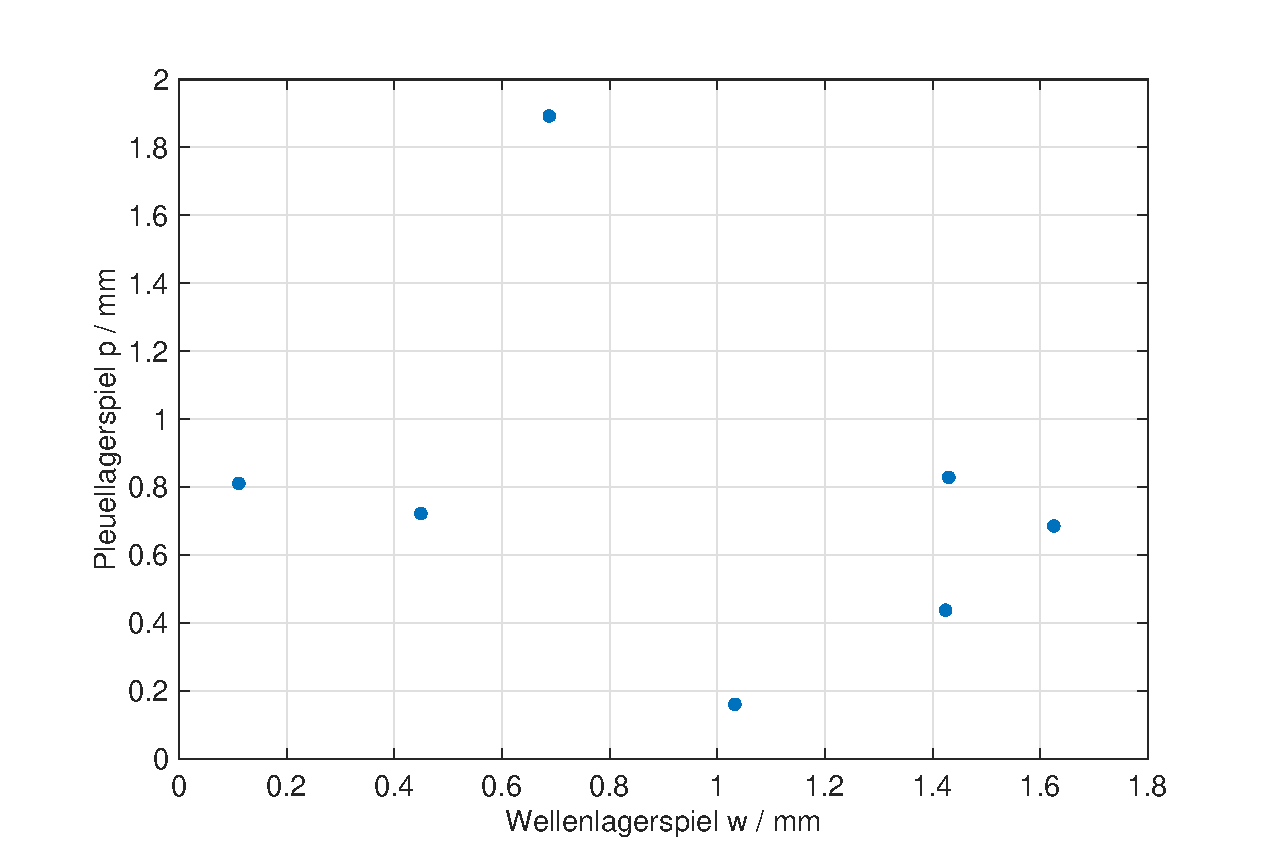
\includegraphics[width=0.5\textwidth]{Kapitel10/Bilder/image4}}
  \caption{Streudiagramm des Lagerspiels eines Motors}
  \label{fig:Lagerspiel}
\end{figure}

\noindent In Bild \ref{fig:Lagerspiel} ist keine eindeutige Tendenz der Messwerte zu erkennen, sodass von einer geringen Korrelation der Messwerte ausgegangen werden kann. Eine n\"{a}here Aussage liefert die numerische Auswertung des Korrelationskoeffizienten r der Stichprobe. Dieser folgt zu

\begin{equation}\label{eq:tensixty}
r=\dfrac{s_{pw}}{s_{p} \cdot s_{w}} =-0.2949
\end{equation}

\noindent Der Korrelationskoeffizient ist leicht negativ. Das hei{\ss}t, dass mit steigendem Wert des Wellenlagerspiels der Wert des Pleuellagerspiels leicht abnimmt. Mit einem Betrag von $r < 0.5$ best\"{a}tigt sich die Annahme einer schwachen Korrelation.\newline

\noindent Mithilfe eines Hypothesentests soll die Signifikanz der Korrelation untersucht werden. Hierzu wird die Hypothese $\rho = 0$ gegen die Alternative $\rho \neq 0$ bei einem Signifikanzniveau von $\alpha = 5 \%$ gepr\"{u}ft. Die Grenzen ergeben sich aus der inversen t-Verteilung mit N -- 2 Freiheitsgraden zu

\begin{equation}\label{eq:tensixtyone}
c_{1} =-2.5706
\end{equation}

\noindent und

\begin{equation}\label{eq:tensixtytwo}
c_{2} =-2.5706
\end{equation}

\noindent Die Bewertungsgr\"{o}{\ss}e t berechnet sich zu

\begin{equation}\label{eq:tensixtythree}
t=r\cdot \sqrt{\dfrac{N-2}{1-r^{2}}} =-0.6901
\end{equation}

\noindent Da der Wert t innerhalb der berechneten Grenzen $c_{1}$ und $c_{2}$ liegt, wird die Hypothese $\rho = 0$ angenommen. Entsprechendes zeigt auch die aus der t-Verteilung mit N -- 2 Freiheitsgraden berechnete Wahrscheinlichkeit von

\begin{equation}\label{eq:tensixtyfour}
p=F(t)=52.09 \%
\end{equation}

\noindent Sie sagt aus, mit welcher Wahrscheinlichkeit eine Korrelation von - 0.2949 auftritt, wenn der Korrelationskoeffizient $\rhoup = 0$ ist. Der Wahrscheinlichkeitswert liegt zwischen den Werten $\alpha/2$ und $1 - \alpha/2$. Die Hypothese $\rho = 0$ wird deshalb nicht verworfen. Die Auswertung mithilfe des Hypothesentestes entspricht der auf Basis des Streudiagrammes vorgenommenen Bewertung.\newline

\noindent Da auch der Konfidenzbereich des Korrelationskoeffizienten zur Bewertung dessen Signifikanz herangezogen werden kann, soll dieser zus\"{a}tzlich berechnet werden. Es gilt

\begin{equation}\label{eq:tensixtyfive}
\tanh \left(\tanh ^{-1} (r)-\dfrac{c_{2} }{\sqrt{N-3}} \right)<\rho \le \tanh \left(\tanh ^{-1} (r)-\dfrac{c_{1}}{\sqrt{N-3}} \right)
\end{equation}

\noindent Mit einer Konfidenzzahl $\gamma = 95 \%$ errechnen sich die ben\"{o}tigten Grenzen $c_{1}$ und $c_{2}$ aus der inversen Standardnormalverteilung zu $c_{1} = - 1.96$ und $c_{2} = 1.96$. Mit dem bereits berechneten Korrelationskoeffizienten der Stichprobe $r = - 0.2949$ und dem Stichprobenumfang von N = 7 berechnet sich der Konfidenzbereich mit

\begin{equation}\label{eq:tensixtysix}
\rho _{1} =\tanh \left(\tanh ^{-1} (r)-\dfrac{c_{2}}{\sqrt{N-3}} \right)=-0.8575
\end{equation}

\noindent und

\begin{equation}\label{eq:tensixtyseven}
\rho _{2} =\tanh \left(\tanh ^{-1} (r)-\dfrac{c_{1}}{\sqrt{N-3}} \right)=0.5890
\end{equation}

\noindent zu

\begin{equation}\label{eq:tensixtyeight}
-0.8575\le \rho \le 0.5896
\end{equation}

\noindent Da der Konfidenzbereich des Korrelationskoeffizienten den Wert $\rhoup = 0$ mit einschlie{\ss}t, best\"{a}tigt der Konfidenzbereich die Aussage des Hypothesentest.\newline

\noindent In MATLAB zeigt sich die Berechnung wie folgt:

\lstinputlisting[caption = {}]{Kapitel10/mat3.m}

\noindent Dabei steht in dem R\"{u}ckgabeparameter R der Funktion die Korrelationsmatrix \textbf{R} f\"{u}r die Gr\"{o}{\ss}en p und w. Der Wahrscheinlichkeitswert P kann dazu verwendet werden, die Signifikanz des Korrelationskoeffizienten r zu \"{u}berpr\"{u}fen. Liegt der Wert P zwischen $\alpha/2$ und $1 - \alpha/2$, kann die Hypothese $\rho = 0$ auf Basis der vorliegenden Stichprobe nicht verworfen werden. In den beiden Zielgr\"{o}{\ss}en RLO und RUP sind die obere beziehungsweise die untere Grenze des Konfidenzbereiches des Korrelationskoeffizienten enthalten.\newline

\noindent Unterschiede bei der Berechnung des Wertes P sind darauf zur\"{u}ckzuf\"{u}hren, dass MATLAB im Widerspruch zu bekannten Literaturstellen mit der t-Verteilung statt der Standardnormalverteilung rechnet. F\"{u}r Stichprobenumf\"{a}nge mit $N > 25$ ist der Unterschied zu vernachl\"{a}ssigen.

\noindent In Python existiert eine Funktion zur Berechnung des Korrelationskoeffizienten und des Hypothesentests f\"{u}r $\rho = 0$, aber es existiert keine Funktion zur Berechnung des Konfidenzbereichs. Die Funktion kann aber mit den Angaben in Tabelle 10.6 selbst implementiert werden.

\lstinputlisting[caption = {}]{Kapitel10/mat4.m}

\subsection{Bewertung des Korrelationskoeffizienten mehrdimensionaler Stichproben}

\noindent \"{A}quivalent zu dem in Abschnitt 10.3.2 eingef\"{u}hrten Konfidenzbereich f\"{u}r den Korrelationskoeffizienten kann auch f\"{u}r Korrelationsmatrizen ein Konfidenzbereich angegeben werden.

\begin{equation}\label{eq:tensixtynine}
\rho _{1jk} \le \rho _{jk} \le \rho _{2jk}
\end{equation}

\noindent Dabei berechnen sich die Werte $\rho_{1jk}$ und $\rho_{2jk}$ wie bei zweidimensionalen Stichproben zu

\begin{equation}\label{eq:tenseventy}
\rho _{1jk} =\tanh \left(\tanh ^{-1} \left(r_{jk} \right)-\dfrac{c_{2} }{\sqrt{N-3} } \right)
\end{equation}

\noindent beziehungsweise

\begin{equation}\label{eq:tenseventyone}
\rho _{2jk} =\tanh \left(\tanh ^{-1} \left(r_{jk} \right)-\dfrac{c_{1} }{\sqrt{N-3} } \right)
\end{equation}

\noindent Der Konfidenzbereich der Korrelationsmatrix kann damit beschrieben werden durch

\begin{equation}\label{eq:tenseventytwo}
\begin{pmatrix}
1 & \rho _{112} & \dots & \rho _{11M}\\
\rho _{121} & 1 & \dots & \rho _{12M}\\
\dots & \dots & \dots & \dots\\
\rho _{1M1} & \rho _{1M2} & \dots & 1\\
\end{pmatrix} \le P \le
\begin{pmatrix}
1 & \rho _{212} & \dots & \rho _{21M}\\
\rho _{221} & 1 & \dots & \rho _{22M}\\
\dots & \dots & \dots & \dots\\
\rho _{2M1} & \rho _{2M2} & \dots & 1\\
\end{pmatrix}
\end{equation}

\noindent Liegt der Wert $\rhoup_{jk}$ = 0 innerhalb des Konfidenzbereiches sind die entsprechenden Datens\"{a}tze nicht signifikant korreliert.\newline

\noindent Da die Gr\"{o}{\ss}en paarweise miteinander verglichen werden, kann auch der Hypothesentest f\"{u}r die Korrelationskoeffizienten durchgef\"{u}hrt werden. Dabei gelten dieselben Annahmen und Herleitungen wir f\"{u}r den Hypothesentest zweidimensionaler Stichproben.\newline

\noindent
\colorbox{lightgray}{%
\arrayrulecolor{white}%
\renewcommand\arraystretch{0.6}%
\begin{tabular}{ wl{16.5cm} }
{\fontfamily{phv}\selectfont
\noindent{Beispiel: Emissionsuntersuchung}}
\end{tabular}%
}\medskip

\noindent F\"{u}r eine Umweltstudie soll die Abh\"{a}ngigkeit der Fahrzeugemissionen E / g/km vom Hubraum H / cm$^{3}$ des PKWs, der Leistung P / kW und der Masse M / kg untersucht werden. Hierzu wurden die in Tabelle \ref{tab:teneight} dargestellten Werte aufgenommenen.

\begin{table}[H]
\setlength{\arrayrulewidth}{.1em}
\caption{Messreihe zur Untersuchung der Emission von Fahrzeugen}
\setlength{\fboxsep}{0pt}%
\colorbox{lightgray}{%
\arrayrulecolor{white}%
\begin{tabular}{ wc{4cm} | wc{4cm} | wc{4cm} | wc{4cm} }
\hline\xrowht{10pt}

\fontfamily{phv}\selectfont\textbf{Hubraum H / cm$^{3}$} &
\fontfamily{phv}\selectfont{Leistung P / kW} &
\fontfamily{phv}\selectfont{Masse M / kg} &
\fontfamily{phv}\selectfont{Emissionen E /g/km} \\\hline \xrowht{10pt}

\fontfamily{phv}\selectfont{1197} &
\fontfamily{phv}\selectfont{63} &
\fontfamily{phv}\selectfont{1205} &
\fontfamily{phv}\selectfont{113} \\\hline \xrowht{10pt}

\fontfamily{phv}\selectfont{1197} &
\fontfamily{phv}\selectfont{81} &
\fontfamily{phv}\selectfont{1210} &
\fontfamily{phv}\selectfont{114} \\\hline \xrowht{10pt}

\fontfamily{phv}\selectfont{1197} &
\fontfamily{phv}\selectfont{81} &
\fontfamily{phv}\selectfont{1229} &
\fontfamily{phv}\selectfont{112} \\\hline \xrowht{10pt}

\fontfamily{phv}\selectfont{1395} &
\fontfamily{phv}\selectfont{81} &
\fontfamily{phv}\selectfont{1382} &
\fontfamily{phv}\selectfont{94} \\\hline \xrowht{10pt}

\fontfamily{phv}\selectfont{1395} &
\fontfamily{phv}\selectfont{81} &
\fontfamily{phv}\selectfont{1382} &
\fontfamily{phv}\selectfont{124} \\\hline \xrowht{10pt}

\fontfamily{phv}\selectfont{1395} &
\fontfamily{phv}\selectfont{81} &
\fontfamily{phv}\selectfont{1395} &
\fontfamily{phv}\selectfont{92} \\\hline \xrowht{10pt}

\fontfamily{phv}\selectfont{1395} &
\fontfamily{phv}\selectfont{81} &
\fontfamily{phv}\selectfont{1395} &
\fontfamily{phv}\selectfont{119} \\\hline \xrowht{10pt}

\fontfamily{phv}\selectfont{1395} &
\fontfamily{phv}\selectfont{192} &
\fontfamily{phv}\selectfont{1225} &
\fontfamily{phv}\selectfont{120} \\\hline \xrowht{10pt}

\fontfamily{phv}\selectfont{1395} &
\fontfamily{phv}\selectfont{92} &
\fontfamily{phv}\selectfont{1249} &
\fontfamily{phv}\selectfont{116} \\\hline \xrowht{10pt}

\fontfamily{phv}\selectfont{1395} &
\fontfamily{phv}\selectfont{110} &
\fontfamily{phv}\selectfont{1268} &
\fontfamily{phv}\selectfont{119} \\\hline \xrowht{10pt}

\fontfamily{phv}\selectfont{1395} &
\fontfamily{phv}\selectfont{110} &
\fontfamily{phv}\selectfont{1293} &
\fontfamily{phv}\selectfont{121} \\\hline \xrowht{10pt}

\fontfamily{phv}\selectfont{1395} &
\fontfamily{phv}\selectfont{110} &
\fontfamily{phv}\selectfont{1288} &
\fontfamily{phv}\selectfont{116} \\\hline \xrowht{10pt}

\fontfamily{phv}\selectfont{1395} &
\fontfamily{phv}\selectfont{110} &
\fontfamily{phv}\selectfont{1270} &
\fontfamily{phv}\selectfont{109} \\\hline \xrowht{10pt}

\fontfamily{phv}\selectfont{1395} &
\fontfamily{phv}\selectfont{110} &
\fontfamily{phv}\selectfont{1296} &
\fontfamily{phv}\selectfont{112} \\\hline \xrowht{10pt}

\fontfamily{phv}\selectfont{1395} &
\fontfamily{phv}\selectfont{110} &
\fontfamily{phv}\selectfont{1290} &
\fontfamily{phv}\selectfont{110} \\\hline \xrowht{10pt}

\fontfamily{phv}\selectfont{1984} &
\fontfamily{phv}\selectfont{162} &
\fontfamily{phv}\selectfont{1351} &
\fontfamily{phv}\selectfont{139} \\\hline \xrowht{10pt}

\fontfamily{phv}\selectfont{1984} &
\fontfamily{phv}\selectfont{162} &
\fontfamily{phv}\selectfont{1370} &
\fontfamily{phv}\selectfont{149} \\\hline \xrowht{10pt}

\fontfamily{phv}\selectfont{1984} &
\fontfamily{phv}\selectfont{169} &
\fontfamily{phv}\selectfont{1382} &
\fontfamily{phv}\selectfont{165} \\\hline \xrowht{10pt}

\fontfamily{phv}\selectfont{1984} &
\fontfamily{phv}\selectfont{169} &
\fontfamily{phv}\selectfont{1402} &
\fontfamily{phv}\selectfont{159} \\\hline \xrowht{10pt}

\fontfamily{phv}\selectfont{1984} &
\fontfamily{phv}\selectfont{221} &
\fontfamily{phv}\selectfont{1476} &
\fontfamily{phv}\selectfont{99} \\\hline \xrowht{10pt}

\fontfamily{phv}\selectfont{1984} &
\fontfamily{phv}\selectfont{221} &
\fontfamily{phv}\selectfont{1495} &
\fontfamily{phv}\selectfont{102} \\\hline \xrowht{10pt}

\fontfamily{phv}\selectfont{1598} &
\fontfamily{phv}\selectfont{81} &
\fontfamily{phv}\selectfont{1299} &
\fontfamily{phv}\selectfont{119} \\\hline \xrowht{10pt}

\fontfamily{phv}\selectfont{1598} &
\fontfamily{phv}\selectfont{81} &
\fontfamily{phv}\selectfont{1317} &
\fontfamily{phv}\selectfont{85} \\\hline \xrowht{10pt}

\fontfamily{phv}\selectfont{1598} &
\fontfamily{phv}\selectfont{81} &
\fontfamily{phv}\selectfont{1432} &
\fontfamily{phv}\selectfont{106} \\\hline \xrowht{10pt}

\fontfamily{phv}\selectfont{1598} &
\fontfamily{phv}\selectfont{81} &
\fontfamily{phv}\selectfont{1265} &
\fontfamily{phv}\selectfont{117} \\\hline \xrowht{10pt}

\fontfamily{phv}\selectfont{1968} &
\fontfamily{phv}\selectfont{110} &
\fontfamily{phv}\selectfont{1354} &
\fontfamily{phv}\selectfont{119} \\\hline \xrowht{10pt}

\fontfamily{phv}\selectfont{1968} &
\fontfamily{phv}\selectfont{110} &
\fontfamily{phv}\selectfont{1375} &
\fontfamily{phv}\selectfont{122} \\\hline \xrowht{10pt}

\fontfamily{phv}\selectfont{1968} &
\fontfamily{phv}\selectfont{135} &
\fontfamily{phv}\selectfont{1394} &
\fontfamily{phv}\selectfont{109} \\\hline \xrowht{10pt}

\fontfamily{phv}\selectfont{1968} &
\fontfamily{phv}\selectfont{135} &
\fontfamily{phv}\selectfont{1449} &
\fontfamily{phv}\selectfont{119} \\\hline \xrowht{10pt}

\fontfamily{phv}\selectfont{1968} &
\fontfamily{phv}\selectfont{135} &
\fontfamily{phv}\selectfont{1377} &
\fontfamily{phv}\selectfont{122} \\\hline

\end{tabular}%
}
\label{tab:teneight}
\end{table}

\clearpage

\noindent Die Daten werden zun\"{a}chst grafisch dargestellt. 

\noindent 
\begin{figure}[H]
  \centerline{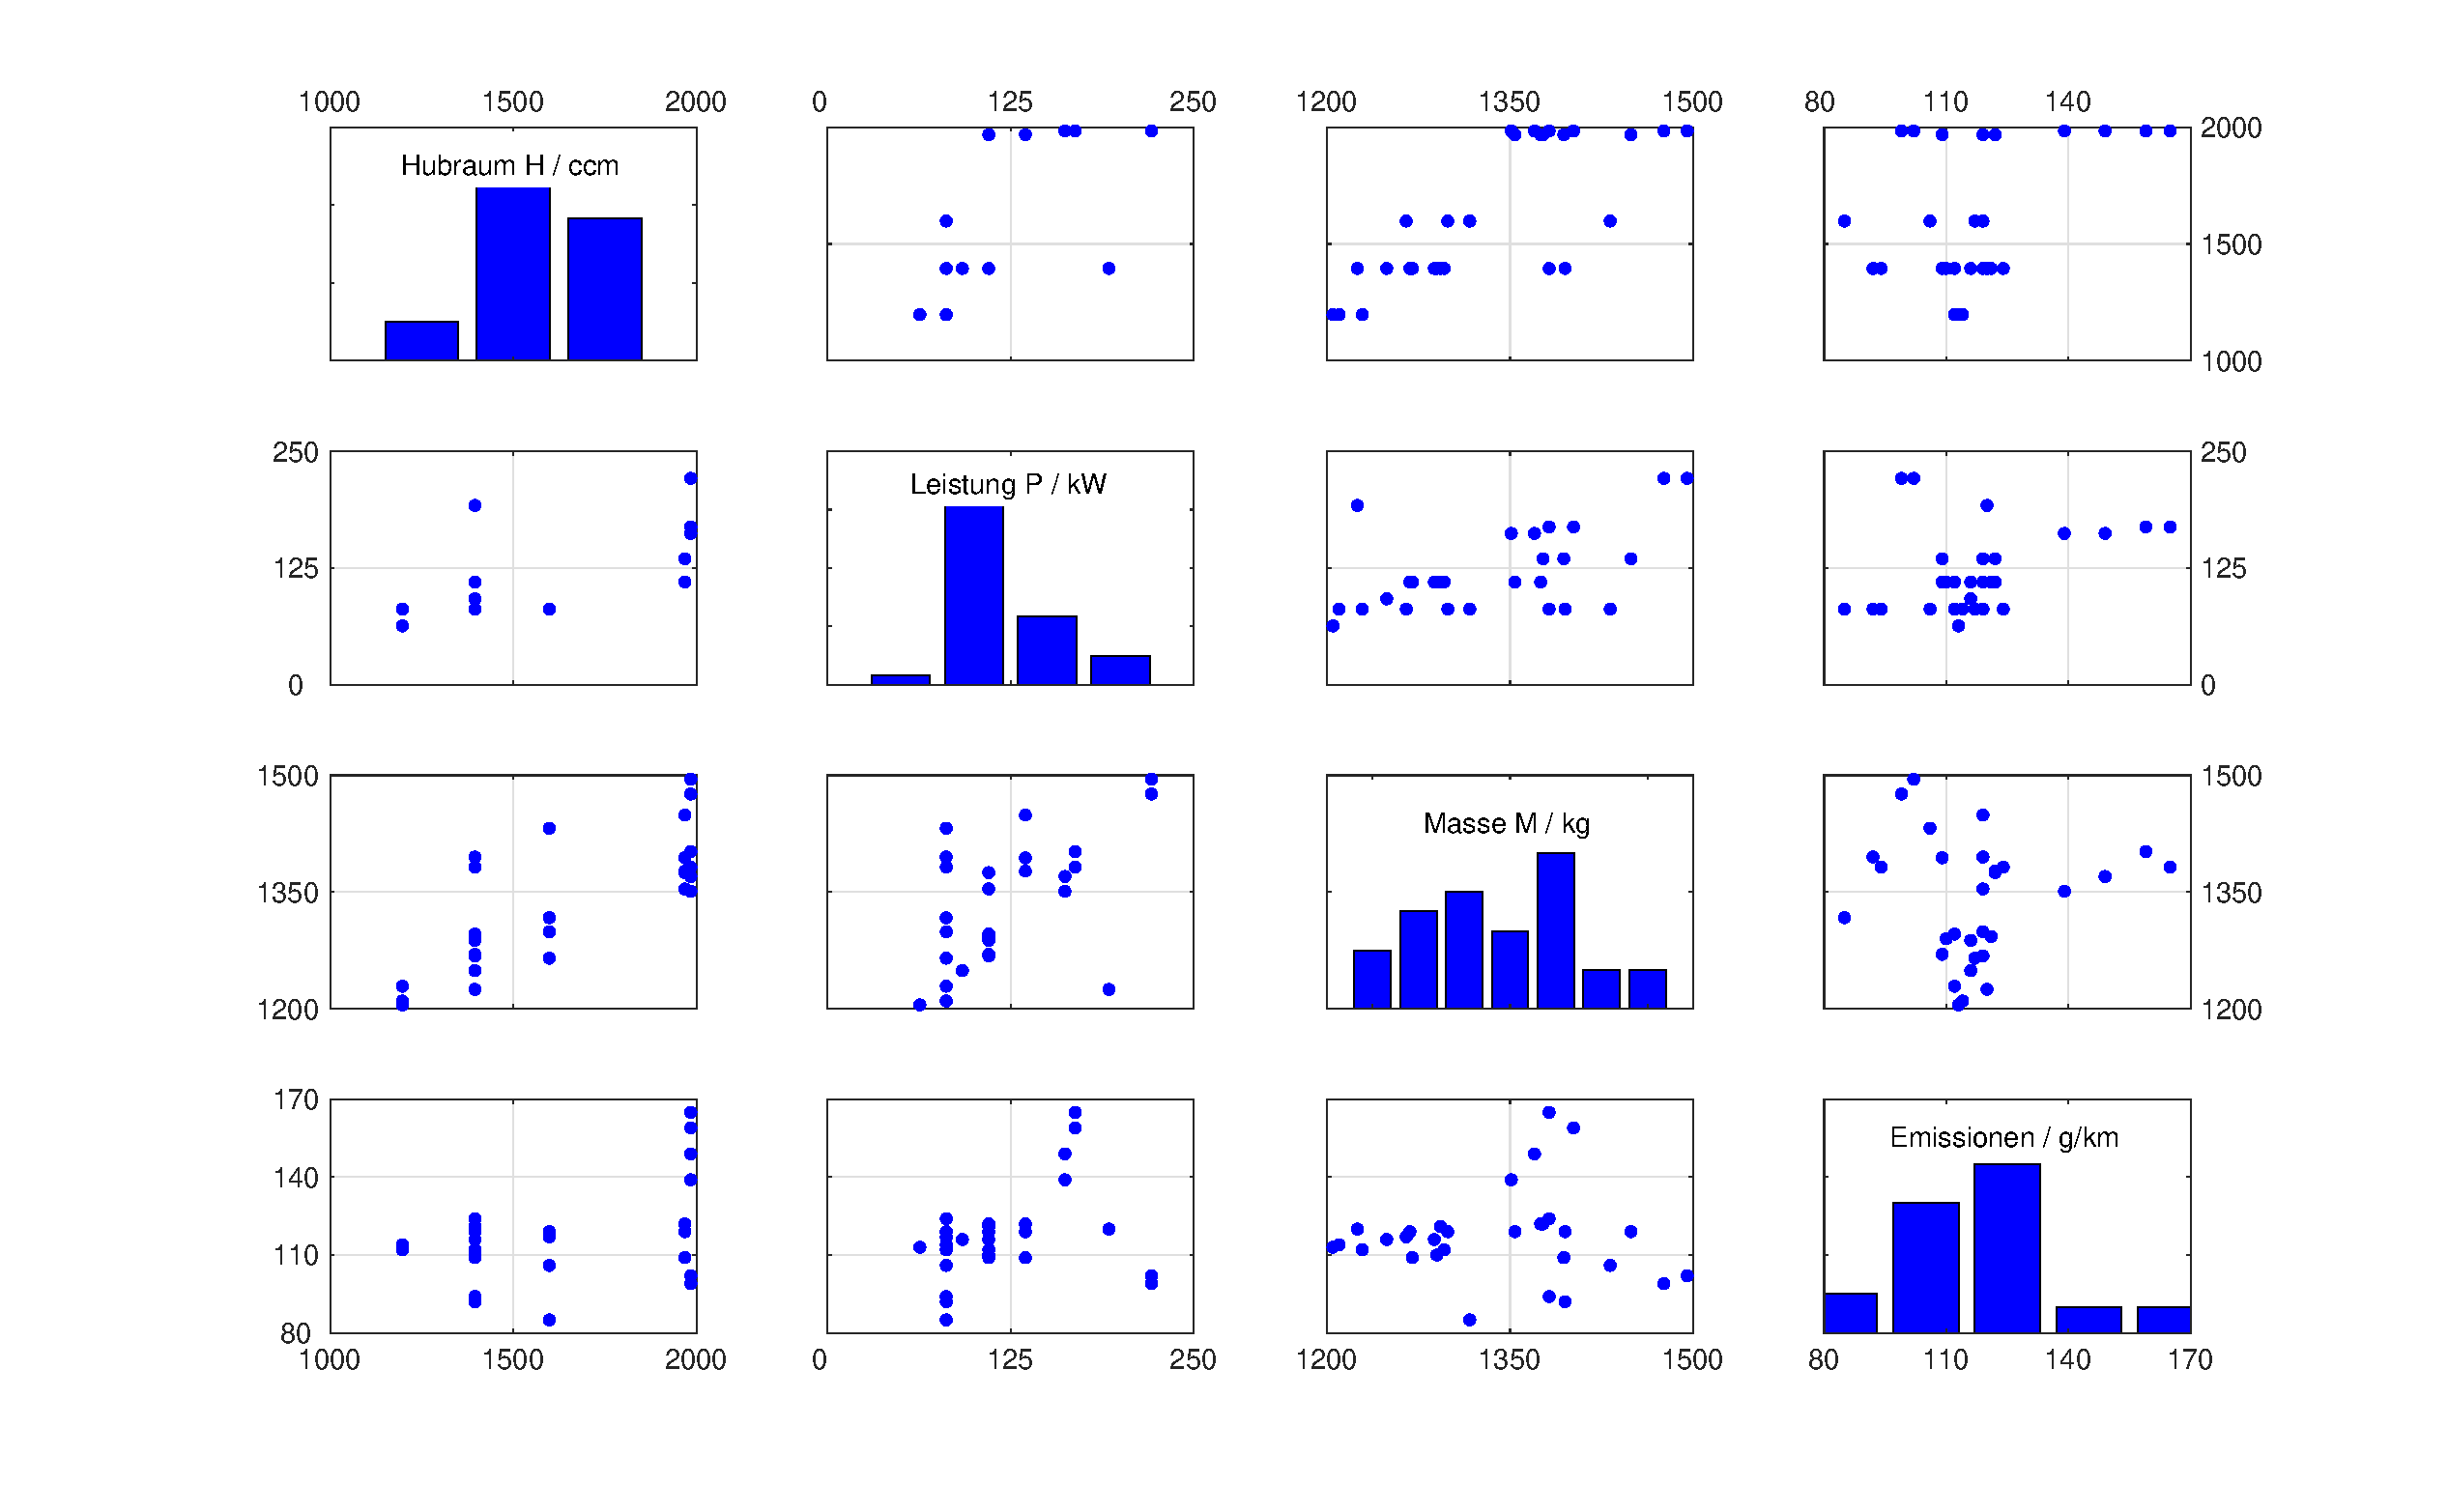
\includegraphics[width=1\textwidth]{Kapitel10/Bilder/image5}}
  \caption{Streudiagramm-Matrix der Messwerte}
  \label{fig:Fahrzeugemissionen}
\end{figure}

\noindent Es ergibt sich die Korrelationsmatrix von 

\begin{equation}\label{eq:tenseventythree}
R=
\begin{pmatrix}
1 & 0.6641 & 0.7122 & 0.4019\\
0.6641 & 1 & 0.4789 & 0.3345\\
0.7122 & 0.4789 & 1 & 0.0261\\
0.4019 & 0.3345 & 0.0261 & 1\\
\end{pmatrix}
\end{equation}

\noindent Zwischen den untersuchten Gr\"{o}{\ss}en existiert nur eine schwache bis mittlere Korrelation. Die h\"{o}chste Korrelation besteht zwischen Hubraum und Masse sowie Hubraum und Leistung. Motoren mit gr\"{o}{\ss}erem Hubraum haben ein h\"{o}heres Gewicht und eine h\"{o}here Leistung. \newline

\noindent F\"{u}r das Beispiel aus Tabelle \ref{tab:teneight} ergibt sich die Wahrscheinlichkeit p daf\"{u}r, dass die Stichproben nicht korreliert sind, gegen die Alternative, dass sie eine von null verschiedene Korrelation haben, von

\begin{equation}\label{eq:tenseventyfour}
P(R=0)=\begin{pmatrix}
0 & 0.0001 & 0.0000 & 0.0277\\
0.0001 & 0 & 0.0074 & 0.0708\\
0.0000 & 0.0074 & 0 & 0.8910\\
0.0277 & 0.0708 & 0.8910 & 0\\
\end{pmatrix}
\end{equation}

\noindent In Kombination mit dem Signifikanzniveau von $\alpha = 0.05$ ergibt sich, dass alle Korrelationen signifikant sind bis auf die Korrelation zwischen Masse und Emissionen sowie Leistung und Emissionen. Zu derselben Aussage kommt die Bewertung des Konfidenzbereiches des Korrelationskoeffizienten. 

\begin{equation}\label{eq:tenseventyfive}
\rho _{1jk} \le \rho _{jk} \le \rho _{2jk}
\end{equation}

\noindent F\"{u}r das Beispiel aus Tabelle 10.8 errechnet sich der Konfidenzbereich zu

\begin{equation}\label{eq:tenseventysix}
\begin{pmatrix}
1 & 0.3994 & 0.4733 & 0.0487\\
0.3994 & 1 & 0.1433 & -0.0293\\
0.4733 & 0.1433 & 1 & -0.3373\\
0.0487 & 0.0293 & -0.3373 & 1\\
\end{pmatrix}
\le  P \le  
\begin{pmatrix}
1 & 0.8266 & 0.8535 & 0.6658\\
0.8266 & 1 & 0.7157 & 0.6201\\
0.8535 & 0.7157 & 1 & 0.3828\\
0.6658 & 0.6201 & 0.3828 & 1\\
\end{pmatrix}
\end{equation}

\noindent Dabei wird folgende MATLAB-Befehlssequenz verwendet.

\lstinputlisting[caption = {}]{Kapitel10/mat5.m}

\noindent Der Wert $\rhoup = 0$ liegt f\"{u}r die Korrelationen von Masse und Emissionen sowie Leistung und Emissionen innerhalb des Konfidenzbereiches, diese Korrelationskoeffizienten sind somit nicht signifikant. Ein Vergleich mit den Ergebnissen des Hypothesentest zeigt, dass sich beide Aussagen entsprechen.\newline

\noindent Nach diesem Datensatz h\"{a}ngen die Fahrzeugemissionen im Wesentlichen von dem Hubraum des Motors ab.\newline

\clearpage

\noindent In Python ist die Berechnung der Korrelationsmatrix ebenfalls m\"{o}glich, der Hypothesentest f\"{u}r $\rho = 0$ kann jedoch nur f\"{u}r zwei Vektoren durchgef\"{u}hrt werden. Die Berechnung des Konfidenzbereichsmuss mit den Angaben in Tabelle \ref{tab:tensix} selbst implementiert werden.

\lstinputlisting[caption = {}]{Kapitel10/mat6.m}

\clearpage

\subsection{Korrelation und Kausalzusammenhang}

\noindent Der Korrelationskoeffizient stellt ein Ma{\ss} f\"{u}r den numerischen Zusammenhang zweier Gr\"{o}{\ss}en dar. H\"{a}ufig wird die Korrelation zweier Gr\"{o}{\ss}en dazu benutzt, einen Hinweis darauf zu bekommen, ob zwei statistische Gr\"{o}{\ss}en urs\"{a}chlich oder kausal miteinander zusammenh\"{a}ngen.\newline

\noindent Ein kleiner Betrag des Korrelationskoeffizienten nahe null weist darauf hin, dass die Gr\"{o}{\ss}en nicht oder nur gering korreliert sind. Damit ist es unwahrscheinlich, dass die beiden untersuchten Gr\"{o}{\ss}en der Stichprobe einen Kausalzusammenhang aufweisen.\newline

\noindent Aus einem gro{\ss}en Betrag des Korrelationskoeffizienten kann auf eine starke numerische Korrelation geschlossen werden. Damit muss aber nicht zwangsweise ein starker Kausalzusammenhang im Sinne von Ursache und Wirkung zwischen den Gr\"{o}{\ss}en bestehen. Ein Kausalzusammenhang kann nur durch eine geeignete Systemanalyse begr\"{u}ndet werden. Der Korrelationskoeffizient von r = 1 best\"{a}tigt, dass die beiden Gr\"{o}{\ss}en linear voneinander abh\"{a}ngig sind, sagt aber nichts \"{u}ber den Proportionalit\"{a}tsfaktor zwischen den Gr\"{o}{\ss}en aus.\newline

\noindent Kann der Kausalzusammenhang nicht best\"{a}tigt werden, wird die Korrelation als Scheinkorrelation zwischen zwei Gr\"{o}{\ss}en bezeichnet. Solche Scheinzusammenh\"{a}nge k\"{o}nnen dadurch entstehen, dass eine mit beiden Gr\"{o}{\ss}en korrelierte dritte Gr\"{o}{\ss}e existiert, die indirekt einen Kausalzusammenhang zwischen den beiden zun\"{a}chst analysierten Gr\"{o}{\ss}en vort\"{a}uscht.\newline

\noindent Ein bekanntes Beispiel dazu ist die Korrelation zwischen dem R\"{u}ckgang der St\"{o}rche im Burgenland und einem R\"{u}ckgang der Anzahl Neugeborener. Diese Ereignisse haben nichts miteinander zu tun - weder bringen St\"{o}rche Kinder noch umgekehrt. Ein gro{\ss}er Korrelationskoeffizient bedeutet, sie sind kausal allenfalls \"{u}ber eine dritte Gr\"{o}{\ss}e miteinander verbunden, etwa \"{u}ber die Verst\"{a}dterung, die sowohl Nistpl\"{a}tze vernichtet als auch Kleinfamilien ohne Kinder f\"{o}rdert.\newline

\noindent Um einen Kausalzusammenhang wirklich herstellen und um Proportionalit\"{a}tsfaktoren bestimmen zu k\"{o}nnen, w\"{a}ren Experimente n\"{o}tig, bei denen ein Faktor experimentell festgelegt wird und die andere Gr\"{o}{\ss}e gemessen wird. In Bereichen, wo solche Experimente oftmals aus Gr\"{u}nden der zu langen Dauer oder zu hoher Kosten nicht m\"{o}glich sind, kommt die Korrelation zum Einsatz. \newline

\noindent Ist es m\"{o}glich Experimente durchzuf\"{u}hren, w\"{u}rden die Ergebnisse mithilfe der Regressionsanalyse bewertet werden. Im Gegensatz zur Korrelation beschreibt die in Kapitel 11 behandelte Regressionsanalyse einen funktionalen Zusammenhang. Die Korrelation beschreibt dagegen lediglich einen statistischen Zusammenhang zwischen den untersuchten Gr\"{o}{\ss}en.

\clearpage

\subsection{Literatur}

\begin{tabular}{|p{0.6in}|p{5.6in}|} \hline 
[Krey91] & Kreyszig, Erwin: Statistische Methoden und ihre Anwendungen\newline 4., unver\"{a}nderter Nachdruck der 7. Auflage\newline Vandenhoeck \& Ruprecht, G\"{o}ttingen, 1991 \\ \hline 
[Fahr96] & Fahrmeir, Ludwig; Hamerle, Alfred; Tutz, Gerhard: Multivariate statistische Verfahren\newline 2., \"{u}berarbeitete Auflage\newline Walter de Gryter \& Co., Berlin \\ \hline 
[Ross06] & Ross, M. Sheldon: Statistik f\"{u}r Ingenieure und Naturwissenschaftler\newline 3. Auflage\newline Spektrum Akademischer Verlag, M\"{u}nchen, 2006 \\ \hline 
[Hart07] & Hartung, Joachim; Elpelt, B\"{a}rbel: Multivariate Statistik\newline 7., unver\"{a}nderte Auflage\newline R. Oldenbourg Verlag, M\"{u}nchen / Wien \\ \hline 
[Papu01] & Papula, Lothar: Mathematik f\"{u}r Ingenieure und Naturwissenschaftler Band 3\newline 4., verbesserte Auflage\newline Vieweg Teubner, Braunschweig / Wiesbaden, 2008 \\ \hline 
\end{tabular}